% =====================================================================
\chapter{PHÂN TÍCH THIẾT KẾ HỆ THỐNG}\label{chap:thietke}
% =====================================================================

Chương này phân tích yêu cầu chức năng (10 use case, \S\ref{chap:usecase}) và phi chức năng
(\S\ref{sec:nfr}) của hệ thống, rồi đi từ tổng thể đến chi tiết: thiết kế phần cứng
(\S\ref{sec:phancung}), kiến trúc triển khai và mạng (\S\ref{sec:trienkhai}), kiến trúc phần
mềm máy chủ (\S\ref{sec:phanlop}), mô hình tác vụ và đồng bộ (\S\ref{sec:tacvu}), các luồng
hoạt động (\S\ref{sec:luong}), máy trạng thái (\S\ref{sec:fsm}) và phân tích chất lượng kiến
trúc (\S\ref{sec:phantich}).

\section{Yêu cầu chức năng}\label{chap:usecase}
Yêu cầu chức năng được mô tả bằng 10 use case: tác nhân, sơ đồ, bảng tổng hợp và đặc tả
chi tiết từng use case (luồng chính, ngoại lệ, kiểm thử tương ứng).

\subsection{Tác nhân}
\begin{table}[H]
\centering\small
\caption{Các tác nhân của hệ thống}\label{tab:actors}
\begin{tabularx}{\linewidth}{@{}lX@{}}
\toprule
\textbf{Tác nhân} & \textbf{Mô tả} \\ \midrule
Người lái xe & Người gửi/lấy xe; dùng thẻ RFID và nhìn màn hình TFT tại bãi. \\
Người vận hành & Bảo vệ hoặc quản lý bãi; dùng trang web trên điện thoại/máy tính để giám sát và điều khiển thanh chắn. \\
Sensor Client & Tác nhân thiết bị: bo ESP8266 đọc cảm biến chỗ đỗ, lửa, nước và gửi dữ liệu lên máy chủ. \\
RFID Client & Tác nhân thiết bị: bo ESP8266 đọc thẻ ở hai cổng và cảm biến nhiệt độ. \\
Đồng hồ hệ thống & Tác nhân thời gian: kích hoạt việc tự đóng thanh chắn, hết hạn hóa đơn/thông báo/lượt thanh toán. \\
SePay & Hệ thống ngoài: dịch vụ đối soát ngân hàng, cho máy chủ đọc các giao dịch chuyển khoản vào tài khoản của bãi qua API HTTPS. \\
\bottomrule
\end{tabularx}
\end{table}

\subsection{Sơ đồ use case}
Hình~\ref{fig:usecase} tổng hợp 10 use case và quan hệ với các tác nhân. Hai tác nhân
thiết bị (bên phải) là nguồn dữ liệu; hai tác nhân con người (bên trái) là người
hưởng lợi; dịch vụ SePay chỉ tham gia UC04 để xác nhận chuyển khoản.

\begin{figure}[H]
\centering
\mmd[1][0.62]{usecase}
\caption{Sơ đồ use case tổng quát (đường nét đứt: sự kiện theo thời gian — tự đóng thanh chắn, hết hạn thông báo)}\label{fig:usecase}
\end{figure}

\subsection{Bảng tổng hợp use case}
\begin{table}[H]
\centering\small
\caption{Tổng hợp 10 use case, nơi hiện thực và bộ kiểm thử tương ứng}\label{tab:uc-summary}
\begin{tabularx}{\linewidth}{@{}l>{\raggedright\arraybackslash}p{4.2cm}>{\raggedright\arraybackslash}X>{\raggedright\arraybackslash}p{3.1cm}@{}}
\toprule
\textbf{Mã} & \textbf{Tên use case} & \textbf{Module chính} & \textbf{Kiểm thử} \\ \midrule
UC01 & Theo dõi chỗ trống tại bãi & \file{lcd\_display.c} & \file{sensor\_client} \\
UC02 & Giám sát bãi qua trang web & \file{http\_server.c}, \file{index.html} & S2, S12 \\
UC03 & Gửi xe bằng thẻ RFID & \file{rfid\_session.c}, \file{servo.c} & \file{rfid\_session}, \file{rfid\_client} \\
UC04 & Lấy xe và thanh toán phí (VietQR) & \file{rfid\_session.c}, \file{payment.c}, \file{sepay\_client.c} & \file{rfid\_session}, \file{payment}, S25–S27 \\
UC05 & Từ chối quẹt sai cổng / bãi đầy & \file{rfid\_session.c}, \file{lcd\_display.c} & \file{rfid\_session} \\
UC06 & Cảnh báo cháy và sơ tán & \file{udp\_server.c}, \file{servo.c}, \file{buzzer.c} & \file{sensor\_client}, S9 \\
UC07 & Giám sát mực nước, cảnh báo ngập & \file{SensorClient.ino}, \file{parking\_state.c} & \file{sensor\_client}, \file{rfid\_session} \\
UC08 & Giám sát nhiệt độ & \file{RFIDClient.ino}, \file{parking\_state.c} & \file{rfid\_client}, \file{rfid\_session} \\
UC09 & Điều khiển thanh chắn thủ công & \file{http\_server.c}, \file{servo.c} & S12, S13 \\
UC10 & Xem nhật ký vào/ra, giá gửi xe và doanh thu & \file{rfid\_session.c}, \file{http\_server.c} & \file{rfid\_session} \\
\bottomrule
\end{tabularx}
\end{table}
\noindent Tên tệp kiểm thử như \file{rfid\_session} chỉ bộ kiểm thử tự động
(Chương~\ref{chap:kiemthu}); S2, S9,\ldots{} là kịch bản kiểm thử trên phần cứng
(Bảng~\ref{tab:systest}).

\subsection{Đặc tả chi tiết}

\begin{usecase}{UC01}{Theo dõi chỗ trống tại bãi}
\item[Tác nhân] Người lái xe (chính); Sensor Client (nguồn dữ liệu).
\item[Mô tả] Người lái nhìn màn hình TFT ở lối vào để biết số chỗ trống và vị trí từng chỗ trống.
\item[Tiền điều kiện] Sensor Client và máy chủ đã kết nối vào mạng Wi-Fi chung của nhóm.
\item[Luồng chính] \begin{enumerate}[nosep,leftmargin=1.3em]
  \item Xe đi vào/ra một ô đỗ, cảm biến IR của ô đó đổi mức logic.
  \item Sensor Client lọc nhiễu: chỉ chấp nhận mức mới khi giữ ổn định 50\,ms.
  \item Ngay khi trạng thái đổi, Sensor Client gửi bản tin \code{parking\_update} (UDP).
  \item Máy chủ kiểm tra bản tin, cập nhật trạng thái chung và đánh thức tác vụ màn hình.
  \item Màn hình vẽ lại: số chỗ trống \code{FREE SPACES x/5} và 5 ô S1–S5 (xanh = trống, đỏ = có xe).
\end{enumerate}
\item[Ngoại lệ] 3a. Mất gói UDP: bản tin nhắc lại sau tối đa 1\,s sẽ cập nhật lại trạng thái.
  3b. Sensor Client im lặng quá 3\,s (mất điện, mất Wi-Fi): màn hình hiện \code{SENSOR OFFLINE}, 5 ô chuyển xám
      \code{----}; trang web báo \code{SENSOR OFFLINE · LAST KNOWN STATE} và làm mờ sơ đồ bãi.
  4a. Bản tin sai định dạng: bị bỏ qua, trạng thái cũ được giữ.
\item[Hậu điều kiện] Màn hình phản ánh đúng trạng thái 5 chỗ đỗ.
\item[Thông số] Debounce 50\,ms; nhắc lại 1\,s; độ trễ hiển thị $\approx$ 0,1\,s.
\end{usecase}

\begin{usecase}{UC02}{Giám sát bãi qua trang web}
\item[Tác nhân] Người vận hành.
\item[Mô tả] Xem trực quan sơ đồ bãi, số chỗ trống, cảm biến và trạng thái thanh chắn trên điện thoại.
\item[Tiền điều kiện] Thiết bị của người vận hành kết nối cùng mạng Wi-Fi chung với máy chủ.
\item[Luồng chính] \begin{enumerate}[nosep,leftmargin=1.3em]
  \item Người vận hành mở \code{http://parking.local}.
  \item Thiết bị phân giải tên bằng mDNS và nhận địa chỉ IP hiện tại của máy chủ.
  \item Máy chủ trả trang web nhúng trong firmware.
  \item Trang web gọi \code{GET /api/parking} mỗi 1\,s và vẽ sơ đồ 5 ô đỗ (ô có xe màu đỏ, ô trống hiện chữ P màu xanh).
\end{enumerate}
\item[Ngoại lệ] 2a. Thiết bị không hỗ trợ \code{.local}: dùng địa chỉ IP in trên log máy chủ.
  4a. Máy chủ mất kết nối: trang hiển thị \code{ESP32 / OFFLINE}.
\item[Hậu điều kiện] Người vận hành thấy trạng thái bãi với độ trễ $\le$ 1\,s.
\end{usecase}

\begin{usecase}{UC03}{Gửi xe bằng thẻ RFID}
\item[Tác nhân] Người lái xe; RFID Client; Đồng hồ hệ thống.
\item[Mô tả] Người lái quẹt thẻ ở cổng vào để được mở thanh chắn và bắt đầu tính giờ.
\item[Tiền điều kiện] Thẻ chưa có phiên gửi xe; bãi còn phiên trống (tối đa 5).
\item[Luồng chính] \begin{enumerate}[nosep,leftmargin=1.3em]
  \item Người lái đưa thẻ vào đầu đọc cổng vào.
  \item RFID Client đọc UID, chuyển thành chuỗi hex in hoa, gửi \code{rfid\_event} với \code{"gate":"in"}.
  \item Máy chủ kiểm tra bản tin và số thứ tự \code{seq}, trả \code{ACK}, tạo phiên mới, lưu thời điểm vào,
        ghi nhật ký \code{IN} và lưu cả bảng phiên vào flash (NVS).
  \item Máy chủ mở thanh chắn cổng vào (90°) và hẹn giờ đóng sau 3\,s.
  \item Hết 3\,s, đồng hồ hệ thống kích hoạt tự đóng thanh chắn.
\end{enumerate}
\item[Ngoại lệ] 1a. Thẻ để yên trên đầu đọc: chỉ gửi một lần trong 2\,s.
  2a. Gói tin bị mất: chưa nhận \code{ACK} sau 300\,ms thì RFID Client gửi lại (tối đa 6 lần);
      nếu máy chủ nhận bản trùng thì chỉ trả \code{ACK}, không mở cổng lần hai.
  3a. Bãi đầy (5 phiên, \emph{hoặc} cảm biến IR báo cả 5 ô có xe) hoặc thẻ đã ở trong bãi: chuyển sang UC05.
  5a. Người vận hành bấm đóng/mở trên web trước khi hết giờ: lệnh thủ công được ưu tiên, hẹn giờ bị hủy.
\item[Hậu điều kiện] Thẻ có phiên hoạt động; thanh chắn đóng lại.
\item[Thông số] Thời gian mở 3\,s; chống đọc lặp 2\,s; tối đa 5 phiên.
\end{usecase}

\begin{usecase}{UC04}{Lấy xe và thanh toán phí}
\item[Tác nhân] Người lái xe; RFID Client; Người vận hành; SePay; Đồng hồ hệ thống.
\item[Mô tả] Người lái quẹt cùng thẻ ở cổng ra; hệ thống tính phí, hiển thị mã VietQR,
  chờ chuyển khoản rồi hiển thị hóa đơn và mở cổng ra.
\item[Tiền điều kiện] Thẻ đang có phiên gửi xe. Đã khai báo tài khoản nhận trong menuconfig;
  nếu chưa, TFT hiện \code{PAY AT BOOTH} thay cho mã QR và cổng ra chỉ mở khi người vận hành bấm \emph{Confirm paid}.
\item[Luồng chính] \begin{enumerate}[nosep,leftmargin=1.3em]
  \item Người lái quẹt thẻ ở đầu đọc cổng ra (\code{"gate":"out"}).
  \item Máy chủ tính thời gian gửi $t$ và phí $\max(1,\lceil t/3600\rceil)\times5000$\,VNĐ,
        chốt phí tại thời điểm này và tạo mã thanh toán \code{PK} + 6 ký tự.
  \item Kết quả \code{AWAITING\_PAYMENT}: thanh chắn vẫn đóng, xe vẫn ``trong bãi''; TFT
        hiện màn hình \code{SCAN TO PAY} gồm mã QR, phí, \code{NOTE <mã>  ID <thẻ>} và
        tài khoản nhận.
  \item Người lái quét QR bằng ứng dụng ngân hàng và chuyển khoản (số tiền và nội dung
        đã điền sẵn).
  \item Tác vụ SePay của máy chủ hỏi vòng mỗi 3\,s, thấy giao dịch có nội dung chứa mã
        và số tiền $\ge$ phí thì hoàn tất thanh toán.
  \item Máy chủ đóng phiên, ghi nhật ký \code{OUT} kèm thời gian và phí, cộng doanh thu.
  \item Màn hình hiển thị hóa đơn: UID, \code{PARK TIME}, \code{FEE VND} trong 60\,s.
  \item Thanh chắn cổng ra mở và tự đóng sau 3\,s.
\end{enumerate}
\item[Ngoại lệ] 1a. Thẻ chưa vào bãi: chuyển sang UC05.
  1b. Quẹt lại cùng thẻ khi đang chờ: hiện lại đúng mã QR cũ (cùng phí, cùng mã) và đếm lại 180\,s.
  1c. Thẻ khác quẹt ở cổng ra khi lượt thanh toán trước còn hiệu lực: TFT báo
      \code{NEXT CAR: WAIT, ONE IS PAYING} ở dòng cuối màn hình QR, nhật ký ghi \code{WAIT · PAYING}.
  5a. Quá 180\,s chưa nhận tiền: TFT báo \code{PAY AT BOOTH / NO TRANSFER YET - SEE OPERATOR}
      trong 30\,s; xe khác được bắt đầu thanh toán. Chuyển khoản đến muộn vẫn hoàn tất lượt này.
  5b. Không có token SePay hoặc mất Internet: mã QR vẫn hiển thị; người vận hành thấy giao
      dịch trong ứng dụng ngân hàng (hoặc thu tiền mặt) và bấm \code{Confirm paid} trên trang web
      (\code{POST /api/payment/confirm}, cần mã PIN), tiếp tục từ bước 6.
\item[Hậu điều kiện] Phiên được giải phóng; nhật ký có bản ghi \code{OUT}; doanh thu được cộng.
\item[Thông số] 5.000\,VNĐ/giờ, làm tròn lên, tối thiểu 1 giờ; hỏi vòng SePay 3\,s; chờ
  chuyển khoản 180\,s; hóa đơn hiển thị 60\,s.
\end{usecase}

\begin{usecase}{UC05}{Từ chối quẹt sai cổng / bãi đầy}
\item[Tác nhân] Người lái xe; RFID Client; Đồng hồ hệ thống.
\item[Mô tả] Hệ thống từ chối các lần quẹt không hợp lệ và hướng dẫn người lái.
\item[Tiền điều kiện] Một trong ba trường hợp: (a) thẻ đã trong bãi nhưng quẹt ở cổng vào;
  (b) thẻ chưa vào nhưng quẹt ở cổng ra; (c) đã đủ 5 phiên, hoặc cả 5 ô đều có xe theo cảm biến IR, mà có thẻ mới quẹt ở cổng vào.
\item[Luồng chính] \begin{enumerate}[nosep,leftmargin=1.3em]
  \item Máy chủ nhận \code{rfid\_event} và xác định kết quả \code{INVALID\_GATE} hoặc \code{FULL}.
  \item Thanh chắn \emph{không} mở.
  \item Màn hình hiển thị thông báo đỏ trong 5\,s: \code{WRONG GATE} kèm gợi ý
        \code{ALREADY INSIDE - USE EXIT GATE} / \code{NOT CHECKED IN - USE ENTRY GATE},
        hoặc \code{PARKING FULL}.
  \item Nhật ký ghi \code{REJECTED · WRONG GATE} hoặc \code{REJECTED · FULL}.
\end{enumerate}
\item[Ngoại lệ] 3a. Đang hiển thị hóa đơn: thông báo được ưu tiên hiển thị, sau 5\,s hóa đơn hiện lại.
  3b. Có lần quẹt hợp lệ ngay sau đó: thông báo cũ bị xóa ngay.
\item[Hậu điều kiện] Trạng thái phiên không đổi.
\end{usecase}

\begin{usecase}{UC06}{Cảnh báo cháy và sơ tán}
\item[Tác nhân] Sensor Client (cảm biến lửa); Người lái xe; Người vận hành.
\item[Mô tả] Khi phát hiện lửa: báo động tại chỗ, trên web và mở thanh chắn để sơ tán.
\item[Tiền điều kiện] Sensor Client đang gửi dữ liệu.
\item[Luồng chính] \begin{enumerate}[nosep,leftmargin=1.3em]
  \item Cảm biến lửa phát hiện ngọn lửa ổn định quá 50\,ms; Sensor Client gửi ngay \code{"fire":true}.
  \item Máy chủ bật còi (GPIO9 mức thấp).
  \item Máy chủ chuyển sang \emph{chế độ cháy}: mở cả hai thanh chắn và giữ mở.
  \item Màn hình chuyển sang giao diện \code{DANGER / FIRE DETECTED / EVACUATE NOW} có ngọn lửa động.
  \item Trang web hiện băng rôn đỏ \code{FIRE DETECTED}.
\end{enumerate}
\item[Ngoại lệ] 3a. Người vận hành bấm đóng thanh chắn: bị từ chối (HTTP 500) trong chế độ cháy.
  5a. Hết lửa (\code{"fire":false}): tắt còi, đóng cả hai thanh chắn, màn hình trở lại bình thường.
\item[Hậu điều kiện] Lối ra vào thông thoáng trong suốt thời gian có lửa.
\end{usecase}

\begin{usecase}{UC07}{Giám sát mực nước, cảnh báo ngập}
\item[Tác nhân] Sensor Client; Người vận hành.
\item[Mô tả] Theo dõi mực nước ngập tại bãi (mô hình tầng hầm).
\item[Luồng chính] \begin{enumerate}[nosep,leftmargin=1.3em]
  \item Sensor Client đọc ADC chân A0 mỗi 250\,ms.
  \item Quy đổi tuyến tính giá trị ADC 20–700 thành 0–40\,mm (giới hạn trên 40\,mm).
  \item Giá trị được gửi trong \code{parking\_update}; máy chủ kiểm tra dải 0–10.000\,mm.
  \item Màn hình (\code{WATER MM}) và web (\code{WATER LEVEL}) hiển thị giá trị.
  \item Khi mực nước đạt 20\,mm, máy chủ bật \emph{cảnh báo ngập}: còi kêu, ô mực nước trên TFT
        chuyển đỏ kèm dòng \code{FLOOD-NO ENTRY}, web hiện băng rôn \code{FLOOD WARNING}, và
        thẻ quẹt ở cổng vào bị từ chối (\code{FLOOD ALARM - ENTRY CLOSED}); xe trong bãi vẫn ra được.
  \item Cảnh báo chỉ tắt khi mực nước xuống tới 15\,mm (trễ 5\,mm để không bật/tắt liên tục).
\end{enumerate}
\item[Ngoại lệ] 3a. Giá trị âm hoặc vượt dải: bản tin bị từ chối.
\item[Hậu điều kiện] Mực nước hiển thị với độ phân giải 0,1\,mm; khi ngập, không có xe mới đi vào.
\item[Thông số] Ngưỡng bật 20\,mm, ngưỡng tắt 15\,mm.
\end{usecase}

\begin{usecase}{UC08}{Giám sát nhiệt độ}
\item[Tác nhân] RFID Client (DHT11); Người vận hành.
\item[Mô tả] Theo dõi nhiệt độ môi trường tại cổng.
\item[Luồng chính] \begin{enumerate}[nosep,leftmargin=1.3em]
  \item RFID Client đọc DHT11 mỗi 5\,s, giữ giá trị hợp lệ gần nhất.
  \item Mỗi lần đọc thành công, RFID Client gửi bản tin \code{climate} riêng (không phụ thuộc
        việc có xe quẹt thẻ); giá trị cũng đi kèm mỗi \code{rfid\_event}.
  \item Máy chủ kiểm tra dải $-40$ đến $125$\,°C, cập nhật trạng thái chung.
  \item Màn hình (\code{TEMP C}) và web (\code{TEMPERATURE}) hiển thị giá trị.
\end{enumerate}
\item[Ngoại lệ] 1a. DHT11 đọc lỗi (NaN): giữ giá trị cũ, không gửi số sai.
\item[Hậu điều kiện] Nhiệt độ trên màn hình và web không cũ hơn 5\,s.
\end{usecase}

\begin{usecase}{UC09}{Điều khiển thanh chắn thủ công}
\item[Tác nhân] Người vận hành.
\item[Mô tả] Mở/đóng từng thanh chắn hoặc cả hai (khẩn cấp) từ trang web.
\item[Luồng chính] \begin{enumerate}[nosep,leftmargin=1.3em]
  \item Người vận hành bấm \code{OPEN}/\code{CLOSE} của cổng vào, cổng ra, hoặc
        \code{EMERGENCY OPEN/CLOSE ALL}.
  \item Trang web gửi yêu cầu \code{POST} tới \code{/api/barrier/\allowbreak<cổng>/\allowbreak<lệnh>} (cổng: \code{in}, \code{out}, \code{all}; lệnh: \code{open}, \code{close}) kèm mã PIN quản trị trong header \code{X-Parking-Key}; nút bị khóa đến khi có phản hồi.
  \item Máy chủ hủy hẹn giờ tự đóng (nếu có) rồi đặt góc servo.
  \item Trang web cập nhật trạng thái \code{OPEN}/\code{CLOSED}.
\end{enumerate}
\item[Ngoại lệ] 2a. Chưa có hoặc sai mã PIN: máy chủ trả 401, trang web hỏi mã PIN một lần
      và nhớ trong trình duyệt. 3a. Đang có cháy mà yêu cầu đóng: bị từ chối, hiển thị lỗi.
\item[Hậu điều kiện] Thanh chắn ở đúng trạng thái người vận hành chọn.
\end{usecase}

\begin{usecase}{UC10}{Xem nhật ký vào/ra và giá gửi xe}
\item[Tác nhân] Người vận hành.
\item[Mô tả] Biết xe nào đang trong bãi, đã gửi bao lâu, phí tạm tính và 10 sự kiện gần nhất.
\item[Luồng chính] \begin{enumerate}[nosep,leftmargin=1.3em]
  \item Trang web gọi \code{GET /api/rfid} mỗi 2\,s.
  \item Máy chủ trả về đơn giá mỗi giờ, danh sách xe trong bãi (UID, giờ vào, phí tạm tính) và
        10 sự kiện mới nhất (vào, ra kèm thời lượng và phí, bị từ chối).
  \item Trình duyệt của người vận hành (đã nhập PIN) gửi giờ thực cho máy chủ qua
        \code{POST /api/time}; từ đó mọi mốc thời gian là giờ Unix.
  \item Trang web so sánh số thẻ trong bãi với số ô có xe theo cảm biến IR; nếu lệch quá 15\,s thì
        hiện cảnh báo vàng \code{CHECK THE LOT}.
\end{enumerate}
\item[Ngoại lệ] 2a. Máy chủ mất điện: phiên, nhật ký và đồng hồ được khôi phục từ flash;
  thời gian mất điện được bù khi trình duyệt gửi lại giờ thực.
\item[Luồng phụ] Ô \code{TODAY} và \code{LAST 7 DAYS} hiện doanh thu, số lượt vào, số lượt ra
  trong ngày (giờ Việt Nam, UTC+7) và 7 ngày gần nhất; số liệu được lưu cùng phiên trong NVS.
\item[Hậu điều kiện] Người vận hành đối soát được tiền thu và xe trong bãi.
\end{usecase}

\section{Yêu cầu phi chức năng}\label{sec:nfr}
\begin{table}[H]
\centering\small
\caption{Yêu cầu phi chức năng và cách đáp ứng}\label{tab:nfr}
\begin{tabularx}{\linewidth}{@{}p{3.1cm}X>{\raggedright\arraybackslash}p{4.4cm}@{}}
\toprule
\textbf{Yêu cầu} & \textbf{Mức cần đạt} & \textbf{Cách đáp ứng} \\ \midrule
Thời gian đáp ứng & Màn hình cập nhật $\le$ 0,2\,s sau khi xe đỗ/rời ô; thanh chắn mở $\le$ 0,5\,s sau khi quẹt thẻ; trang web $\approx$ 1\,s & Gửi theo thay đổi, vẽ theo sự kiện, tác vụ ưu tiên cao cho UDP \\
An toàn & Có cháy: mở cả hai thanh chắn và bật còi ngay; có ngập: không cho xe vào & Chế độ cháy có ưu tiên cao nhất, bỏ qua lệnh đóng thủ công \\
Độ tin cậy & Không mất lượt quẹt thẻ khi mất gói; không mất xe đang gửi khi mất điện; tự kết nối lại Wi-Fi & ACK và gửi lại, lưu phiên vào NVS, tự kết nối lại \\
Tài nguyên & Chạy trong $\approx$ 321\,KB DRAM của ESP32-C3 cùng ảnh màn hình 115\,KB và TLS & Bộ đệm TLS cấp phát động, trả bộ đệm ảnh động khi thanh toán \\
Bảo mật & Thao tác điều khiển cần mã PIN; bí mật không nằm trong mã nguồn & PIN qua header, cấu hình trong \file{sdkconfig}/\file{secrets.h} \\
Dễ sử dụng & Xem trên mọi điện thoại, không cần cài ứng dụng; trả tiền bằng app ngân hàng bất kỳ & Trang web tại \code{parking.local}, mã VietQR \\
Chi phí và bảo trì & Linh kiện phổ thông; mã nguồn kiểm thử được khi không có phần cứng & Bộ kiểm thử tự động 397 phép trên máy tính \\
\bottomrule
\end{tabularx}
\end{table}


\section{Thiết kế phần cứng}\label{sec:phancung}
\subsection{Mô hình thực tế và bố trí phần cứng}\label{sec:mohinh}
Hình~\ref{fig:model} là mô hình nhóm đã chế tạo. Đế và vách làm bằng bìa formex
trắng (nhẹ, dễ cắt khoét lỗ cho cảm biến, cách điện); 5 ô đỗ được kẻ vạch dọc vách
sau; phía trước là sân quay đầu và hai làn ra/vào nằm hai bên hộp điều khiển ở giữa.

\begin{figure}[H]
\centering
\begin{subfigure}[t]{0.52\linewidth}\centering
  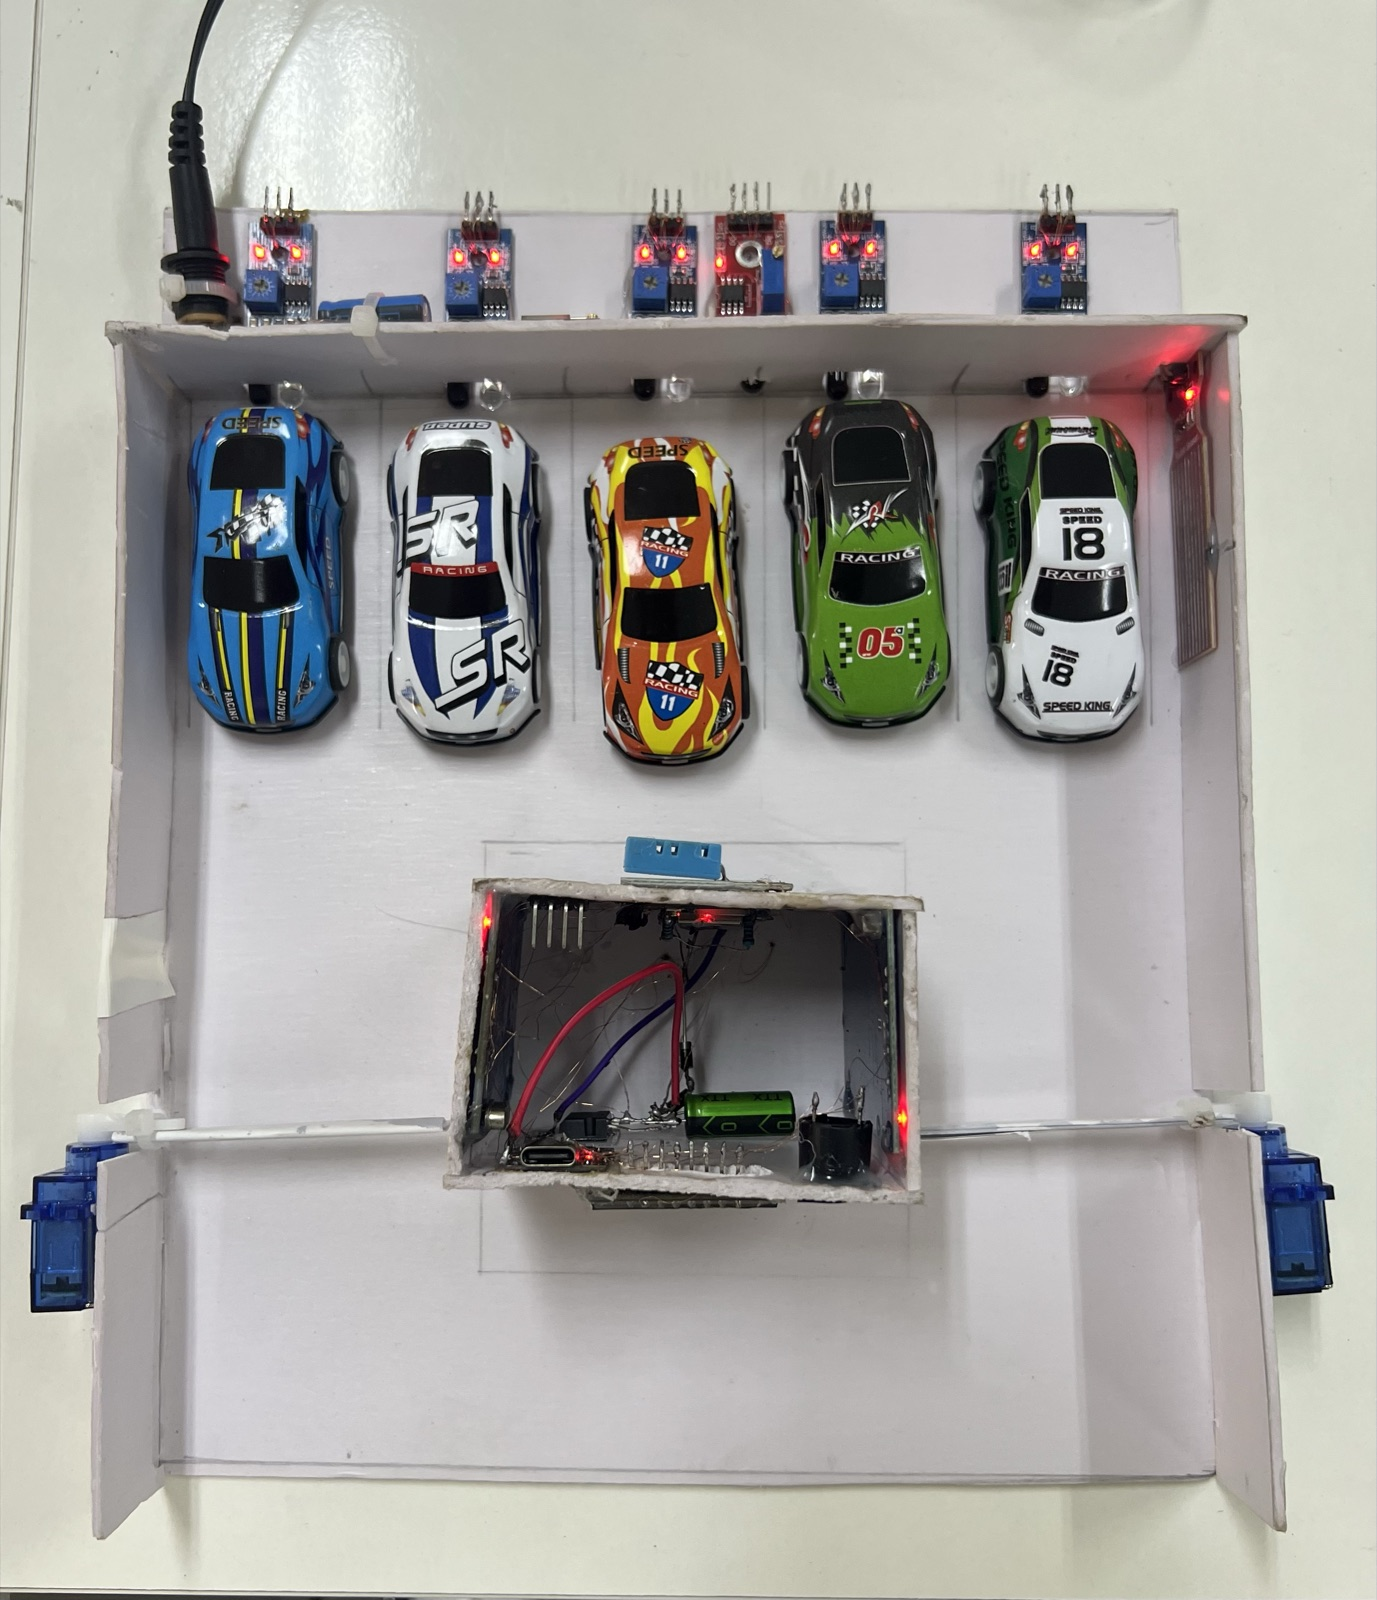
\includegraphics[width=\linewidth,height=0.4\textheight,keepaspectratio]{photos/model_top.jpg}
  \caption{Nhìn từ trên xuống khi bãi có 5 xe: dãy cảm biến trên vách sau, hộp điều khiển ở giữa, hai servo ở hai cổng}\label{fig:model-top}
\end{subfigure}\hfill
\begin{subfigure}[t]{0.45\linewidth}\centering
  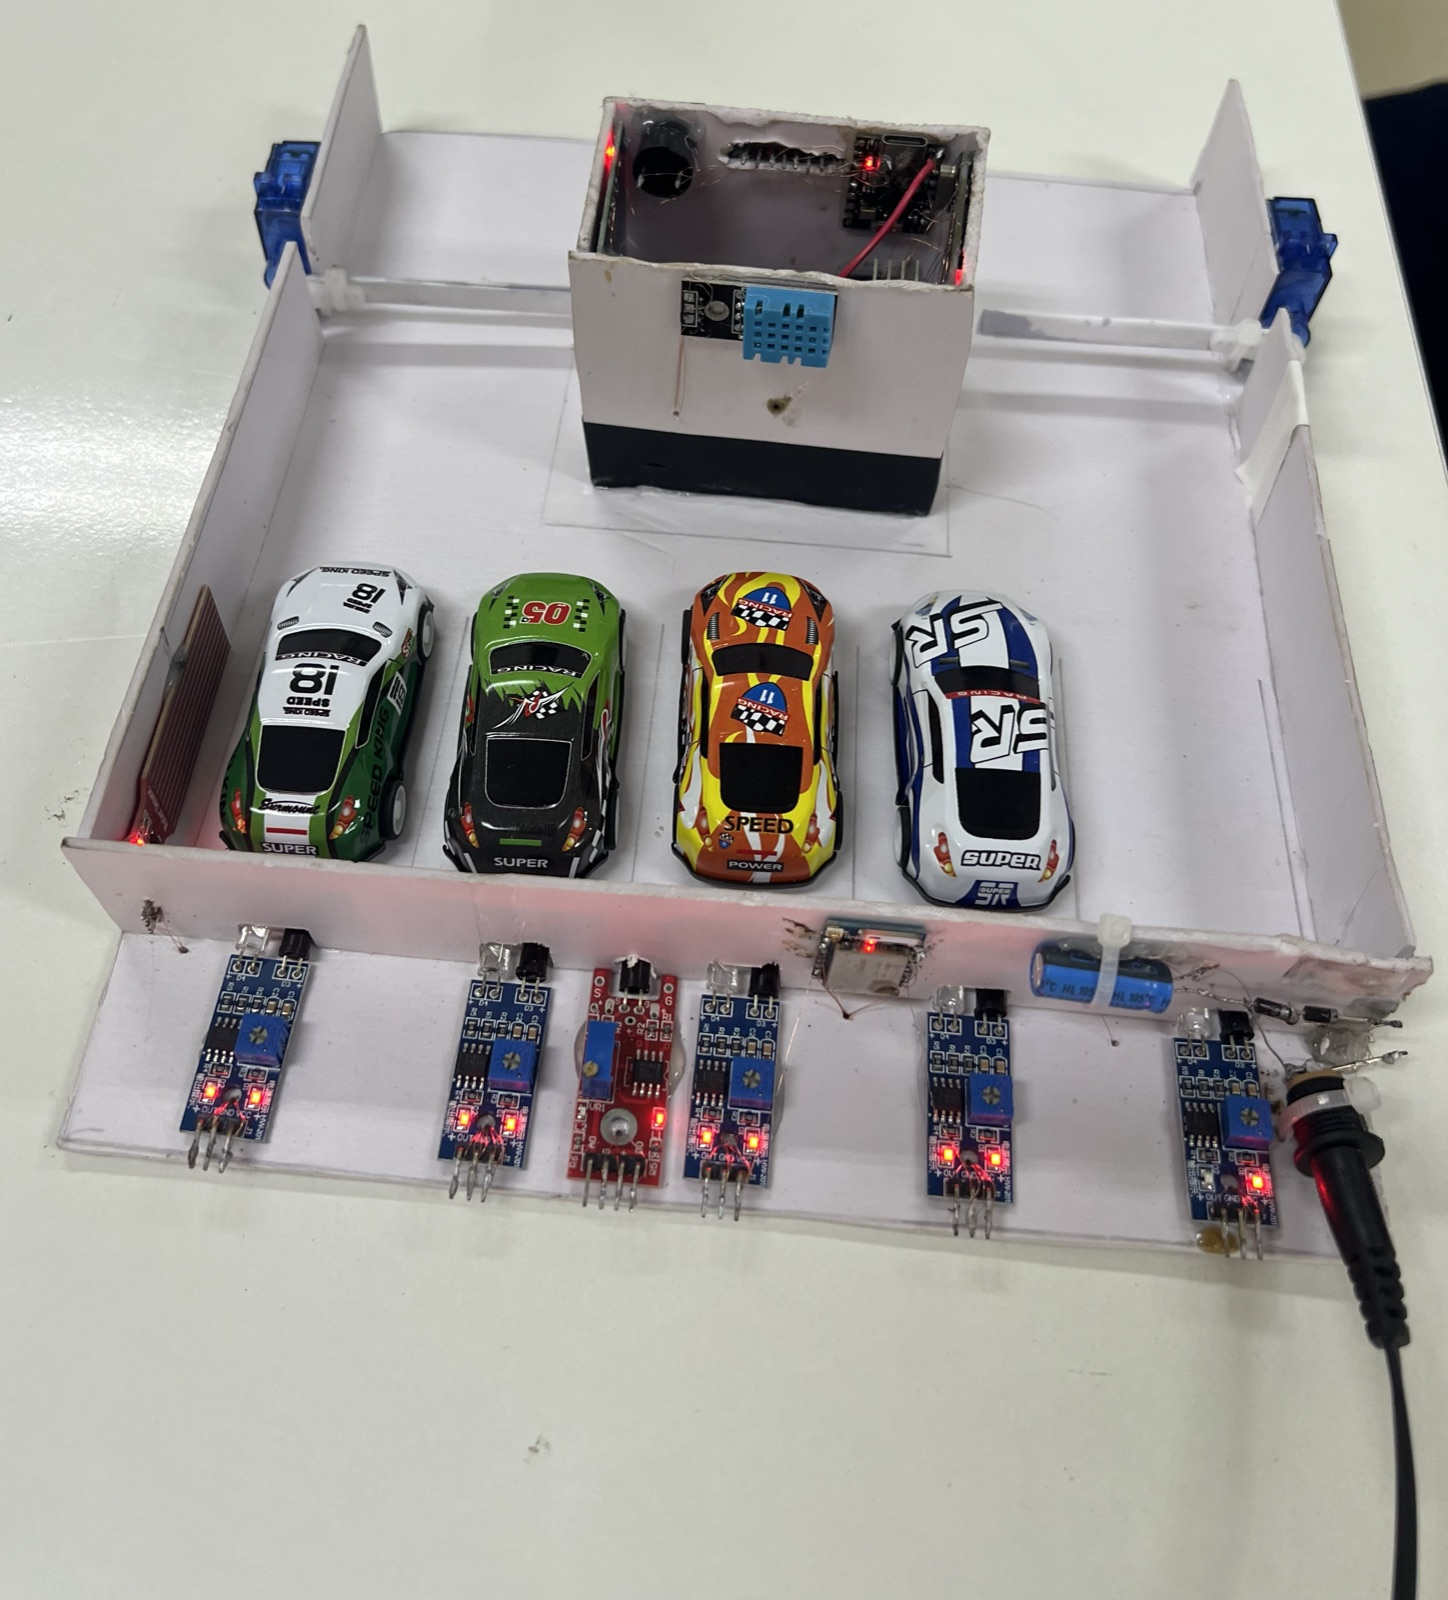
\includegraphics[width=\linewidth,height=0.4\textheight,keepaspectratio]{photos/model_angle.jpg}
  \caption{Mặt ngoài vách sau: 5 module IR HW-201, module lửa (đỏ), jack nguồn DC, diode và tụ lọc; cảm biến nước ở góc trong}\label{fig:model-wall}
\end{subfigure}

\vspace{4pt}
\begin{subfigure}[t]{0.49\linewidth}\centering
  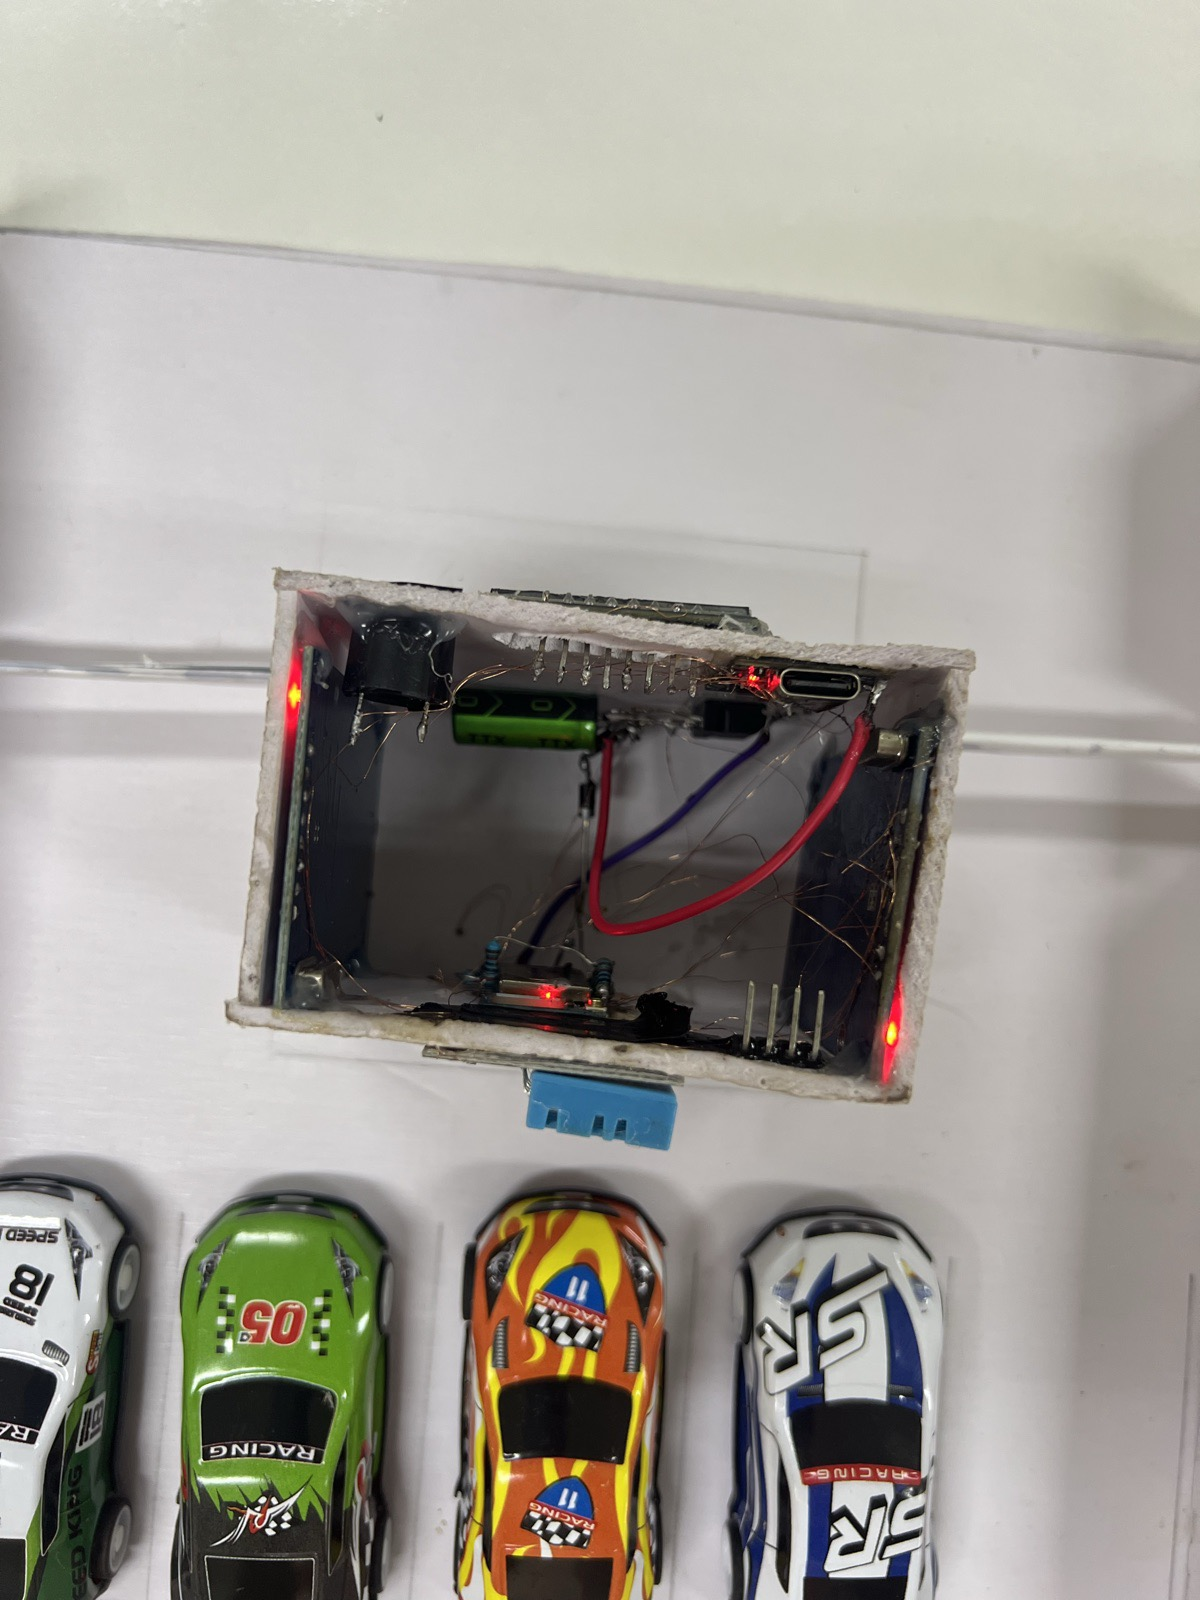
\includegraphics[width=\linewidth,height=0.3\textheight,keepaspectratio]{photos/model_box.jpg}
  \caption{Bên trong hộp điều khiển: bo mạch có cổng USB-C, còi, tụ lọc; đầu đọc RC522 ở hai thành hộp; DHT11 gắn bên ngoài}\label{fig:model-box}
\end{subfigure}\hfill
\begin{subfigure}[t]{0.49\linewidth}\centering
  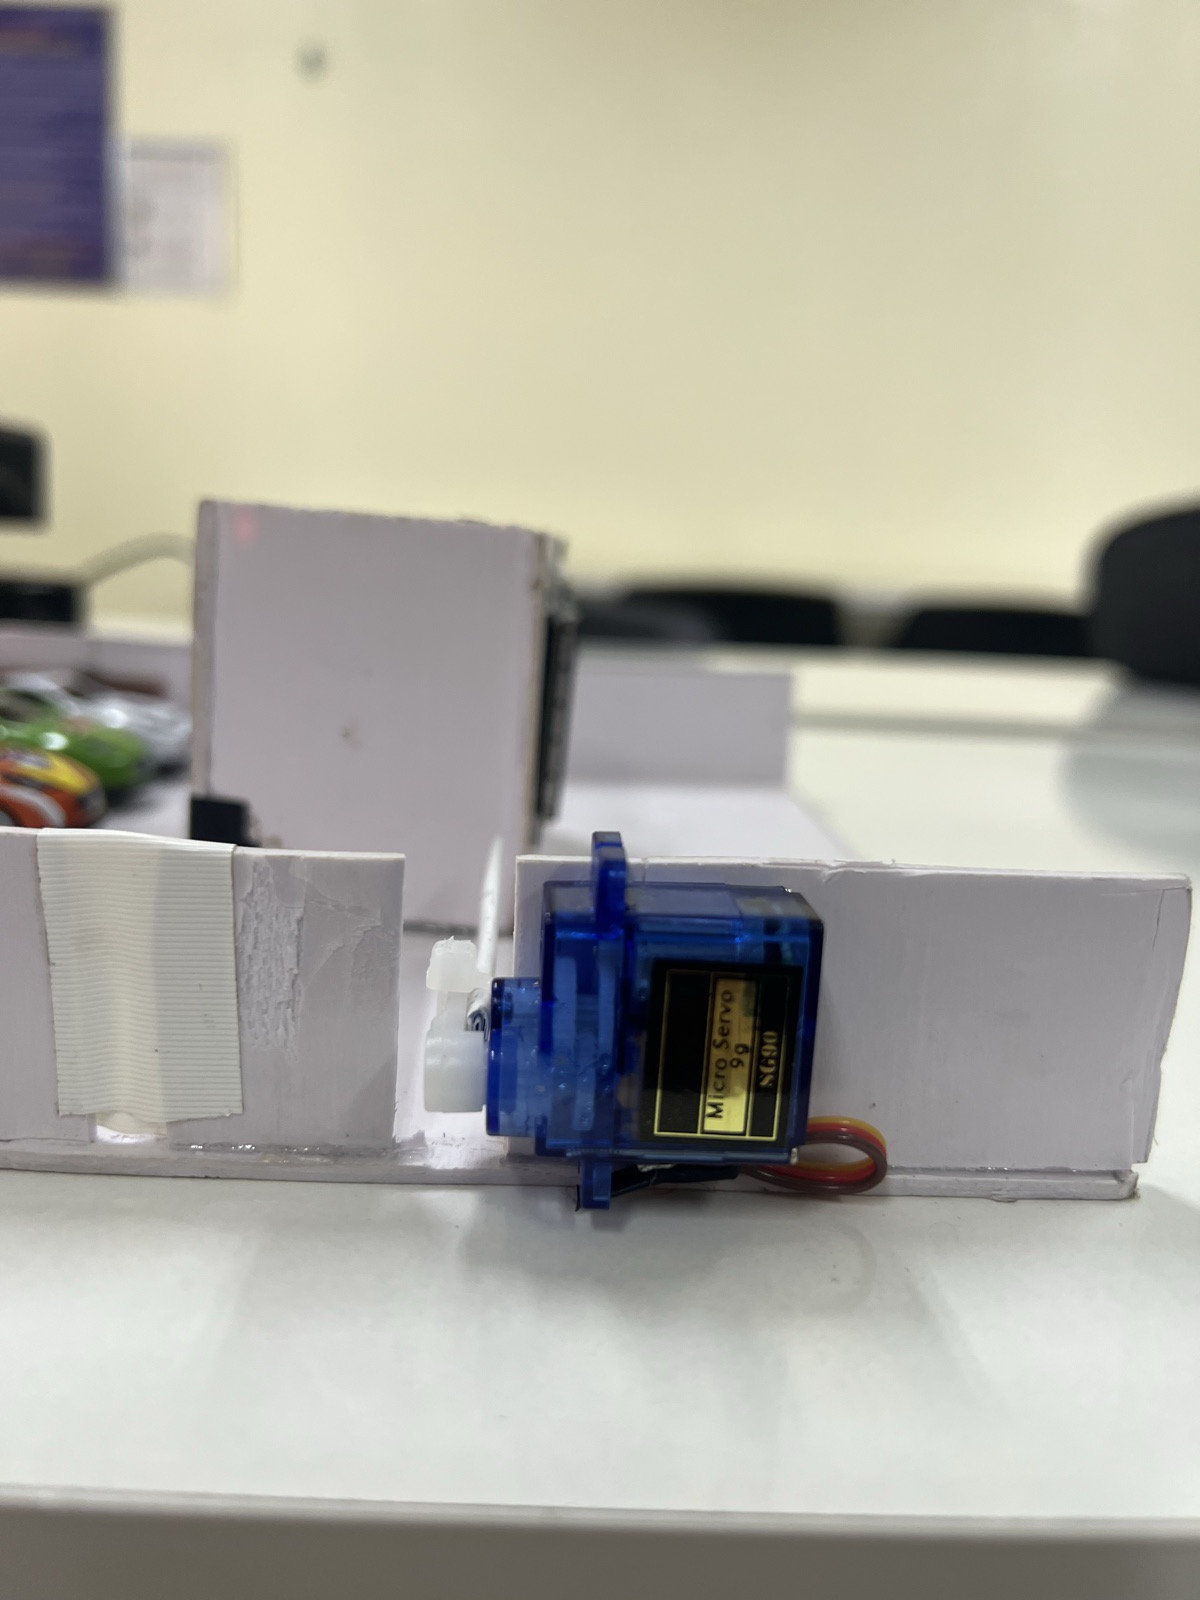
\includegraphics[width=\linewidth,height=0.3\textheight,keepaspectratio]{photos/model_servo.jpg}
  \caption{Servo SG90 gắn ở đầu vách, trục quay cần chắn ngang làn xe}\label{fig:model-servo}
\end{subfigure}
\caption{Mô hình bãi đỗ xe thông minh của nhóm}\label{fig:model}
\end{figure}

\begin{table}[H]
\centering\small
\caption{Vị trí lắp đặt từng thiết bị trên mô hình và lý do}\label{tab:placement}
\begin{tabularx}{\linewidth}{@{}p{3.1cm}p{4.3cm}X@{}}
\toprule
\textbf{Thiết bị} & \textbf{Vị trí} & \textbf{Lý do} \\ \midrule
5 module IR HW-201 & Mặt \emph{ngoài} vách sau, mỗi ô một module; LED phát/thu xuyên qua lỗ khoét, hướng vào đúng giữa ô & Dây và bo mạch nằm ngoài nên lòng bãi gọn, xe không vướng; khoảng cách tới đuôi xe chỉ vài cm, đúng tầm đo của IR. Mỗi module có biến trở chỉnh ngưỡng riêng theo độ phản xạ thực tế \\
Module lửa & Giữa dãy IR, đầu thu hướng vào lòng bãi & Góc nhìn $\approx$ 60° phủ được cả 5 ô từ vị trí trung tâm \\
Cảm biến mực nước & Góc trong của vách sau, sát sàn & Nước thường đọng trước ở điểm thấp và góc tường; đặt sát sàn để phát hiện sớm \\
Hộp điều khiển & Giữa bãi, giữa hai làn & Dây tới cảm biến, đầu đọc và servo đều ngắn; bảo vệ bo mạch khỏi va chạm \\
TFT ST7789 & Mặt trước hộp, quay ra cổng & Người lái nhìn thấy số chỗ trống, hóa đơn và cảnh báo ngay khi tới cổng \\
2 đầu đọc RC522 & Hai hông hộp, mỗi đầu đọc quay ra một làn & Người lái quẹt thẻ từ trong xe ở đúng làn của mình; hai đầu đọc cách nhau bằng chiều rộng hộp nên ít nhiễu chéo \\
2 servo SG90 & Đầu vách trái và phải, cần chắn quay ngang làn & Trục servo nằm ngoài làn, cần chắn nhẹ (nhựa) nên mô-men 1,8\,kg$\cdot$cm là quá đủ \\
DHT11 & Mặt ngoài thành hộp điều khiển & Nằm ngoài lòng hộp để không đo nhầm nhiệt do bo mạch tỏa ra \\
Jack DC, diode, tụ hóa & Mặt ngoài vách sau, cạnh dãy cảm biến & Một điểm cấp nguồn cho cả mô hình; xem đoạn ``Nguồn điện'' \\
\bottomrule
\end{tabularx}
\end{table}

\subsection{Sơ đồ chân}
\begin{table}[H]
\centering\small
\caption{Sơ đồ chân máy chủ ESP32-C3}\label{tab:pin-srv}
\begin{tabularx}{\linewidth}{@{}llX@{}}
\toprule
\textbf{Tín hiệu} & \textbf{GPIO} & \textbf{Ghi chú} \\ \midrule
TFT SCK / MOSI & 4 / 6 & SPI2 qua GPIO matrix; màn hình không cần MISO \\
TFT DC / RST / CS & 7 / 3 / 10 & Chọn lệnh–dữ liệu, reset, chọn chip \\
TFT đèn nền & 5 & Tắt khi khởi tạo để không hiển thị ảnh rác, bật sau khi sẵn sàng \\
Servo cổng vào / ra & 0 / 1 & Chân thường (bo không dùng thạch anh 32\,kHz) \\
Còi & 9 & Tích cực mức thấp; GPIO9 là chân strapping có kéo lên, trùng với trạng thái ``im lặng'' \\
\bottomrule
\end{tabularx}
\end{table}

\begin{table}[H]
\centering\small
\caption{Sơ đồ chân Sensor Client và RFID Client (ESP8266)}\label{tab:pin-clients}
\begin{tabularx}{\linewidth}{@{}llX@{}}
\toprule
\textbf{Tín hiệu} & \textbf{GPIO} & \textbf{Ghi chú} \\ \midrule
\multicolumn{3}{@{}l}{\itshape Sensor Client} \\
Ô đỗ S1–S5 & 16, 4, 14, 13, 12 & Tránh chân strapping (0, 2, 15) và UART (1, 3) \\
Cảm biến lửa (DO) & 5 & Module nhóm sử dụng cho mức cao khi có lửa \\
Mực nước & A0 & Chân ADC duy nhất của ESP8266 \\ \midrule
\multicolumn{3}{@{}l}{\itshape RFID Client} \\
SPI SCK / MOSI / MISO & 14 / 13 / 12 & SPI phần cứng, dùng chung cho 2 đầu đọc \\
SS đầu đọc cổng vào & 5 (D1) & Mỗi thiết bị SPI cần chân chọn chip riêng \\
SS đầu đọc cổng ra & 4 (D2) & \\
RST chung & 16 (D0) & Dùng chung để tiết kiệm chân \\
DHT11 & 2 (D4) & GPIO2 cần mức cao khi khởi động, module DHT11 có sẵn điện trở kéo lên \\
\bottomrule
\end{tabularx}
\end{table}

\subsection{Sơ đồ nguyên lý}\label{sec:schematic}
Các Hình~\ref{fig:sch-server}, \ref{fig:sch-sensor} và \ref{fig:sch-rfid} là sơ đồ nguyên lý
của ba mạch, với các chân GPIO trùng với Bảng~\ref{tab:pin-srv} và \ref{tab:pin-clients}.
Mỗi bản vẽ thể hiện một mạch kèm đầu vào 5\,V riêng (J\_PWR1--3). Trên hai mạch ESP8266, hai
diode 1N4007 mắc nối tiếp hạ 5\,V xuống khoảng 3,6\,V (mỗi diode sụt khoảng 0,7\,V) để cấp
cho ESP8266 và các module của mạch đó; trên mạch máy chủ, servo dùng 5\,V có tụ 100\,µF
riêng, còn màn hình và còi dùng 3,3\,V từ bo ESP32-C3.

\begin{landscape}
\begin{figure}[p]
\centering
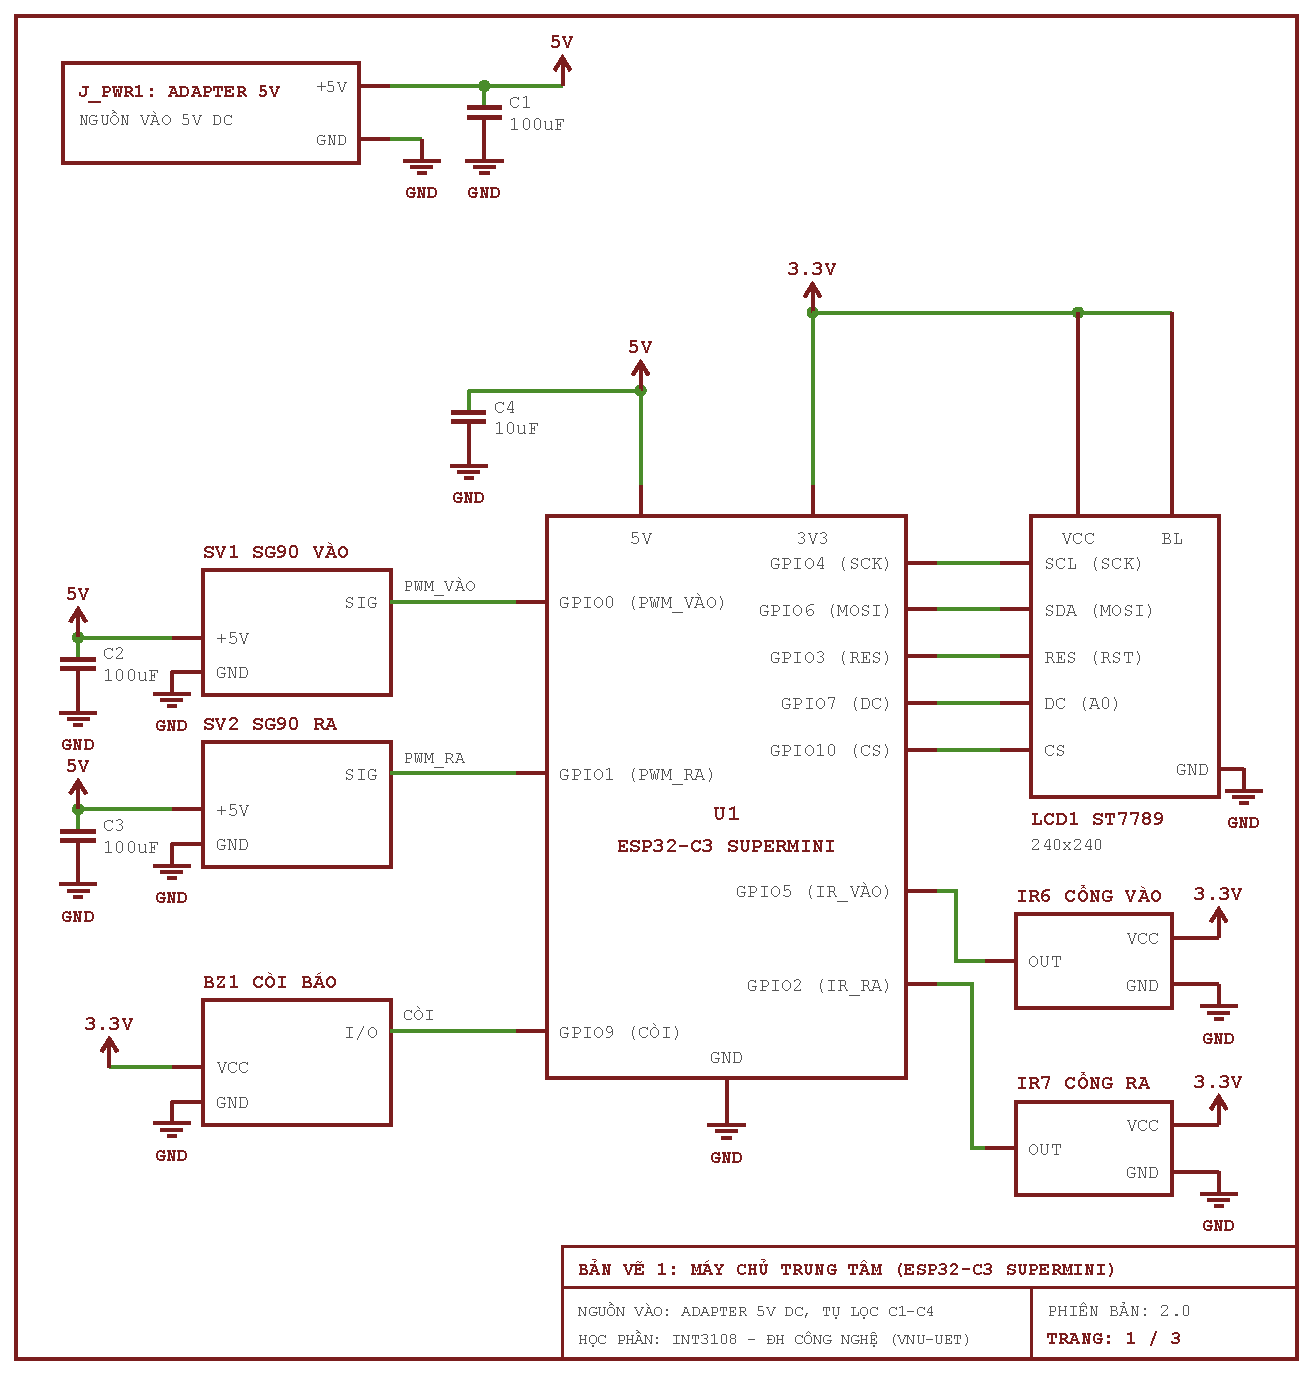
\includegraphics[width=\linewidth]{schematic/sheet1.pdf}
\caption{Sơ đồ nguyên lý máy chủ: ESP32-C3 SuperMini, màn hình ST7789, 2 servo SG90 và còi}\label{fig:sch-server}
\end{figure}
\begin{figure}[p]
\centering
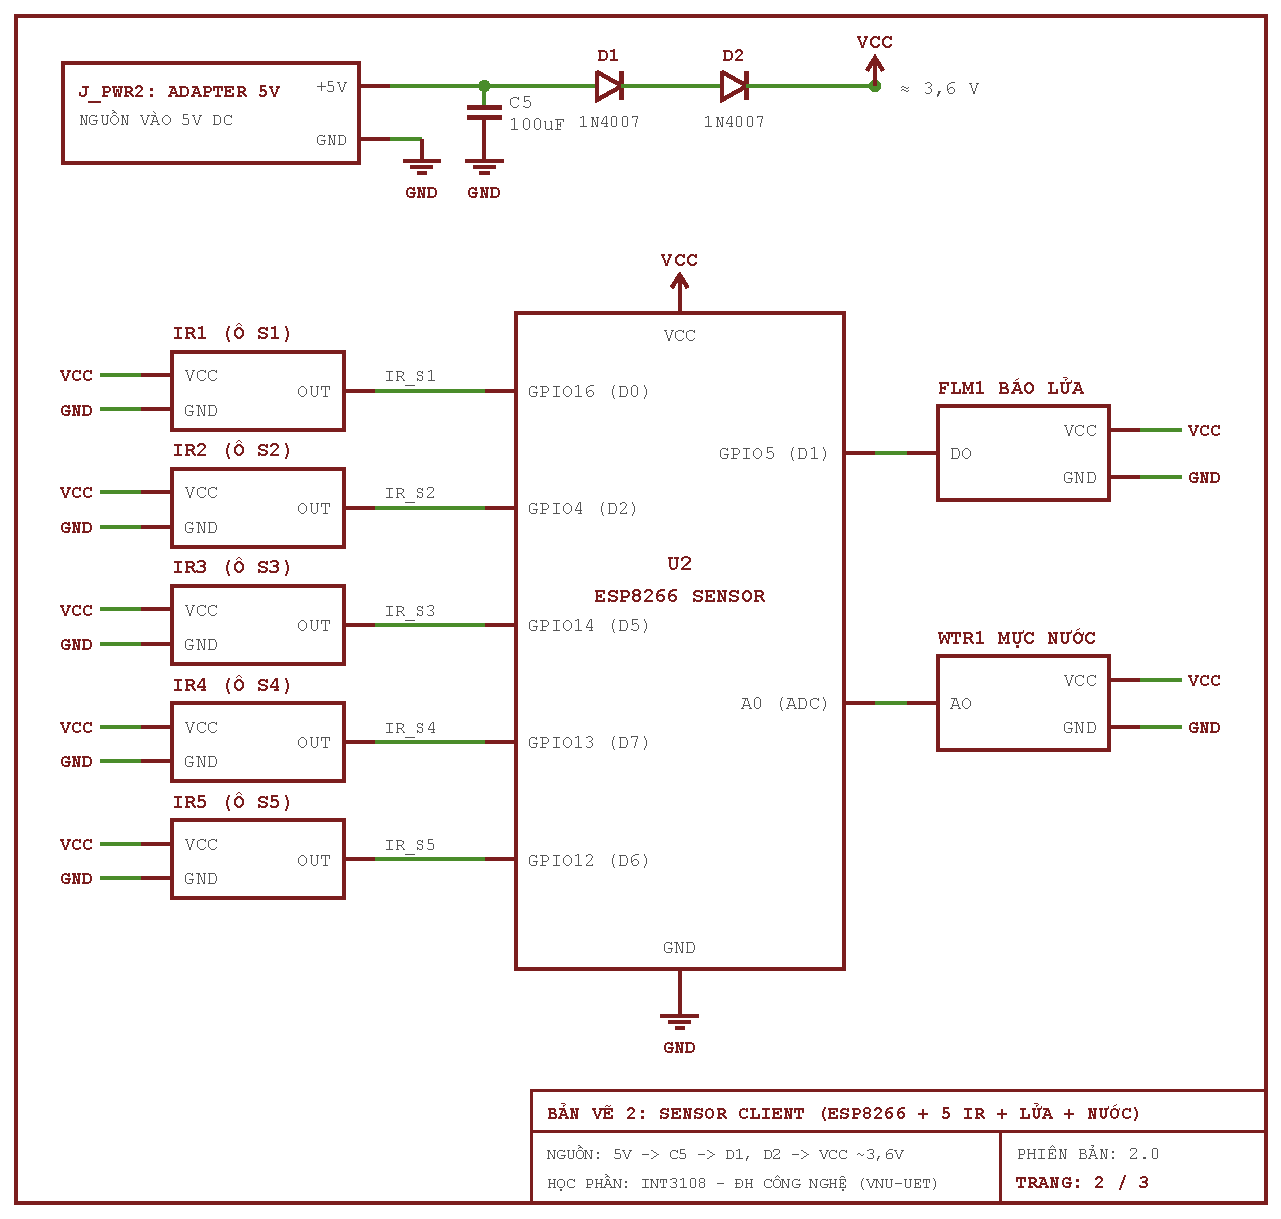
\includegraphics[width=\linewidth]{schematic/sheet2.pdf}
\caption{Sơ đồ nguyên lý Sensor Client: ESP8266, 5 cảm biến hồng ngoại, cảm biến lửa và mực nước}\label{fig:sch-sensor}
\end{figure}
\begin{figure}[p]
\centering
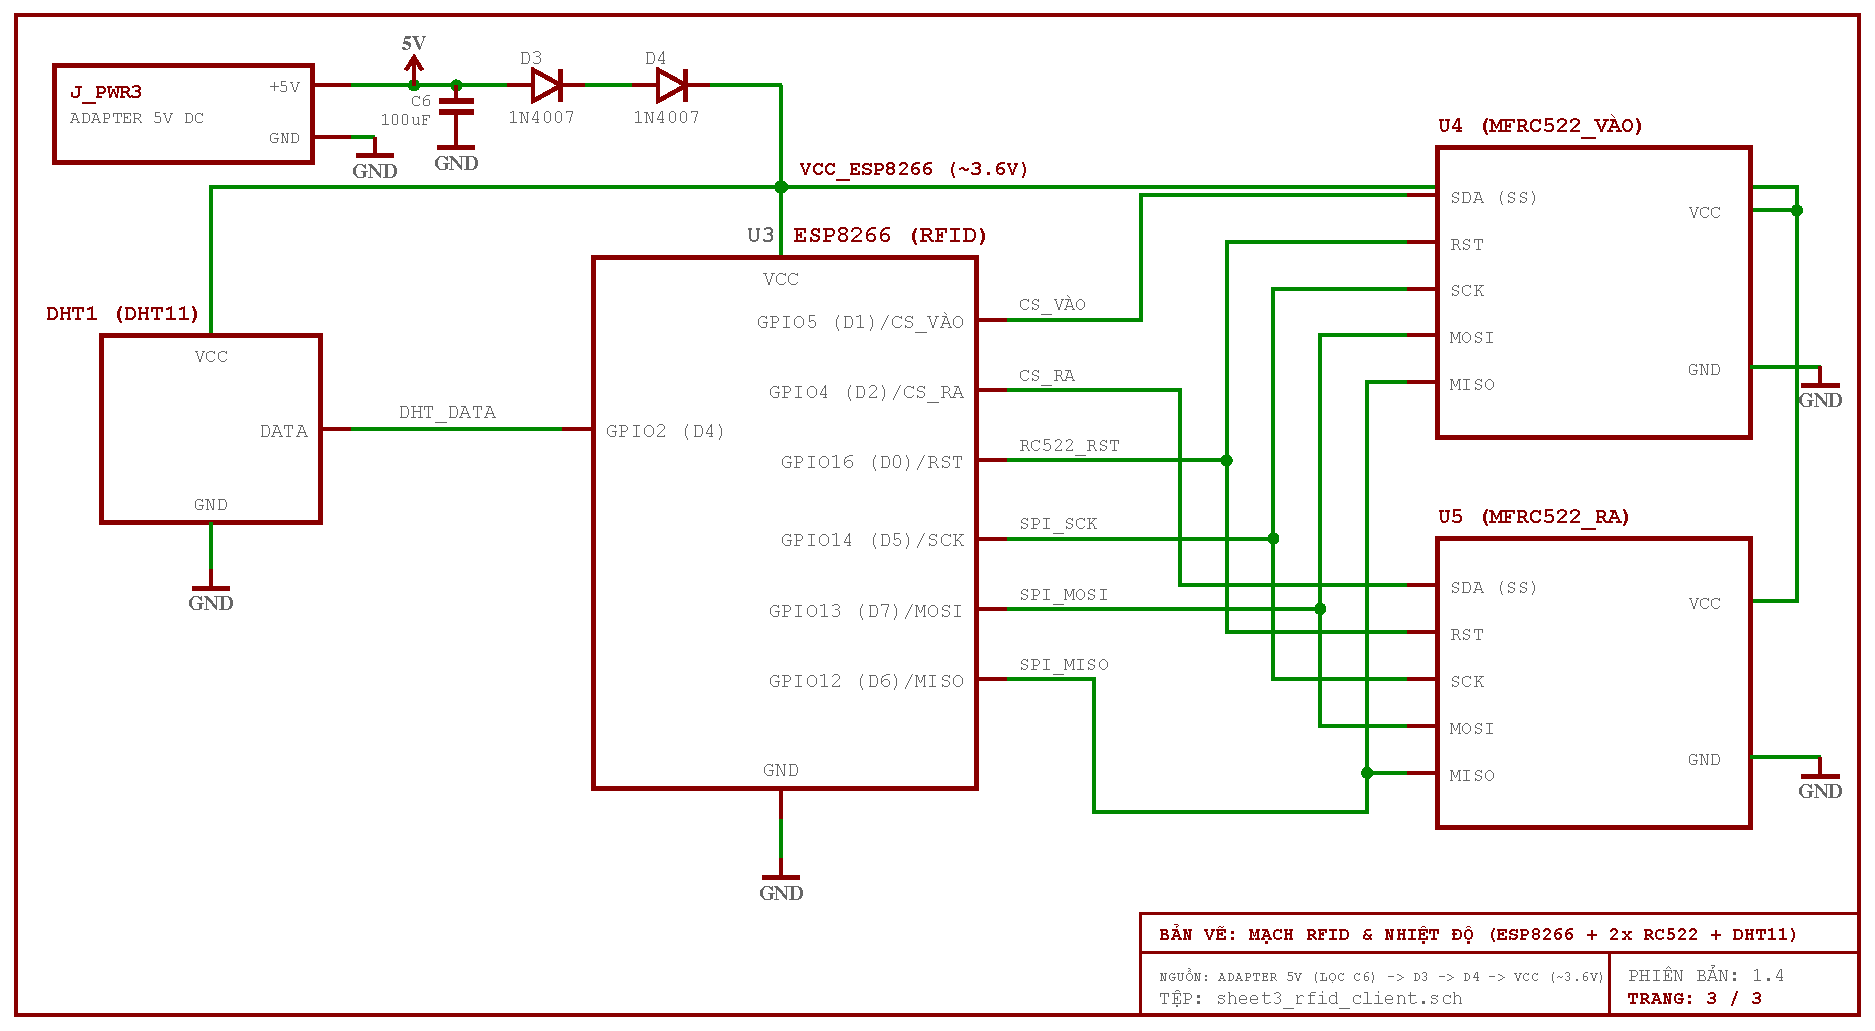
\includegraphics[width=\linewidth]{schematic/sheet3.pdf}
\caption{Sơ đồ nguyên lý RFID Client: ESP8266, 2 đầu đọc RC522 dùng chung SPI và DHT11}\label{fig:sch-rfid}
\end{figure}
\end{landscape}

\paragraph{Nguồn điện.} Mô hình có một điểm cấp nguồn là jack DC trên vách sau
(Hình~\ref{fig:model-wall}); khi trình diễn có thể cấp qua cáp USB vào hộp điều
khiển. Ba chi tiết được thêm sau khi đo thực tế:
\begin{itemize}[nosep]
  \item \textbf{Diode nối tiếp} ở đầu vào: cắm ngược cực bộ nguồn thì diode chặn dòng, không
        làm hỏng ba bo mạch và các module.
  \item \textbf{Tụ hóa lớn} mắc song song với nguồn 5\,V: servo SG90 kéo vài trăm mA lúc khởi
        động; tụ cấp dòng tức thời này nên điện áp không sụt làm ESP32-C3 hay ESP8266
        reset khi thanh chắn chuyển động.
  \item \textbf{Servo lấy nguồn 5\,V}, không lấy từ chân 3V3 của bo (bộ ổn áp trên bo
        chỉ cấp được vài trăm mA), và \textbf{nối chung GND} với ESP32-C3 để xung PWM có cùng
        mức tham chiếu.
\end{itemize}

\section{Kiến trúc triển khai và mạng}\label{sec:trienkhai}
\begin{figure}[H]
\centering
\mmd[1][0.6]{deploy}
\caption{Kiến trúc triển khai: máy chủ, hai client và điện thoại cùng là trạm của mạng Wi-Fi chung có Internet; máy chủ ra Internet để hỏi SePay}\label{fig:deploy}
\end{figure}

Hình~\ref{fig:deploy} cho thấy cấu trúc mạng hình sao quanh router (hoặc điểm phát
trên điện thoại) của nhóm: không bo nào phát điểm truy cập, cả ba bo và điện thoại
của người vận hành đều là trạm Wi-Fi. Bảng~\ref{tab:netparams} liệt kê thông số mạng.
Hai client gửi tới địa chỉ \emph{broadcast giới hạn} \code{255.255.255.255} nên không
cần biết dải mạng hay IP máy chủ; người dùng truy cập bằng tên \code{parking.local}
nên cũng không cần biết IP. Router còn cho máy chủ đường ra Internet để kiểm tra
chuyển khoản qua SePay (mục~\ref{sec:vietqr}). Vì tất cả đều là trạm và tự kết nối
lại, thứ tự bật nguồn các bo không còn quan trọng.

\begin{table}[H]
\centering\small
\caption{Thông số mạng}\label{tab:netparams}
\begin{tabularx}{\linewidth}{@{}lX@{}}
\toprule
SSID / mật khẩu & Tên và mật khẩu mạng Wi-Fi chung của nhóm; mặc định \code{ESP32-Parking} / \code{12345678}. Máy chủ: \code{idf.py menuconfig → Parking network and security}; hai client: \file{secrets.h} \\
Điểm truy cập & Router hoặc điểm phát Wi-Fi (điện thoại) của nhóm, có Internet, cấp IP bằng DHCP; phải \emph{tắt} chế độ cô lập thiết bị (AP/client isolation) \\
Máy chủ & Trạm Wi-Fi, IP do DHCP cấp, tên \code{parking.local}, dịch vụ \code{\_http.\_tcp} cổng 80 \\
UDP & Máy chủ nghe cổng 3333; client gửi tới \code{255.255.255.255:3333}; máy chủ trả ACK (unicast) cho sự kiện quẹt thẻ \\
HTTP & Cổng 80: trang web, \code{/api/parking}, \code{/api/barrier}, \code{/api/rfid}, \code{/api/time}, \code{/api/payment/confirm}; lệnh POST cần mã PIN \\
\bottomrule
\end{tabularx}
\end{table}

\begin{lydo}[Tại sao dùng chung một mạng Wi-Fi có Internet và máy chủ dùng mDNS]
Một mạng Wi-Fi chung (router hoặc điểm phát của nhóm) cho máy chủ \textbf{đường ra
Internet} để hỏi SePay xem đã nhận được chuyển khoản chưa — điều không làm được khi
mạng do một bo ESP8266 tự phát. ESP32-C3 chỉ là trạm nên \textbf{không tốn RAM} cho bộ
đệm từng trạm và DHCP server, dành RAM cho màn hình và TLS. Điện thoại của người vận
hành vốn đã ở trong mạng đó nên mở \code{parking.local} ngay mà không phải đổi Wi-Fi.
Đổi lại, bãi \textbf{phụ thuộc vào router} đó; một số router/điểm phát bật chế độ
\emph{cô lập thiết bị} (AP/client isolation) chặn gói broadcast giữa các thiết bị — chế độ
này phải tắt. Mất Internet thì bãi vẫn chạy, chỉ việc xác nhận chuyển khoản chuyển sang
người vận hành. IP máy chủ do DHCP cấp và có thể thay đổi; mDNS giải quyết bằng một
tên cố định \code{parking.local}. Máy chủ còn \emph{chủ động thông báo lại} tên này mỗi
khi nhận địa chỉ mới (sự kiện \code{IP\_EVENT\_STA\_GOT\_IP}), kể cả khi DHCP đổi địa chỉ
mà không mất kết nối, nên các thiết bị khác không bao giờ giữ một IP cũ.
\end{lydo}

\subsection{Giao thức truyền: UDP broadcast}
\begin{table}[H]
\centering\small
\caption{So sánh giao thức truyền dữ liệu cảm biến}\label{tab:proto}
\begin{tabularx}{\linewidth}{@{}lXXX@{}}
\toprule
& \textbf{UDP} & \textbf{HTTP/TCP} & \textbf{MQTT} \\ \midrule
Thiết lập kết nối & Không & Bắt tay 3 bước & Cần broker \\
Overhead/bản tin & 8 byte & Vài trăm byte & 2+ byte trên TCP \\
Bộ nhớ máy chủ & 1 socket, đệm 256\,B & Socket + đệm mỗi kết nối & Thêm broker \\
Khi mất gói & Mất, bản tin sau bù lại & Tự truyền lại & Có QoS \\
\bottomrule
\end{tabularx}
\end{table}

\begin{lydo}
Sensor Client gửi \textbf{toàn bộ trạng thái} (không phải ``sự kiện thay đổi''), và
nhắc lại mỗi giây. Mất một gói chỉ làm trễ tối đa 1\,s, không làm sai trạng thái lâu
dài, nên độ tin cậy của TCP là không cần thiết, trong khi chi phí của nó (bắt tay,
socket, bộ đệm) đáng kể trên vi điều khiển. Gửi broadcast giới hạn
\code{255.255.255.255} giúp client không cần biết dải mạng của router hay IP máy chủ
và cho phép máy tính trong mạng ``nghe'' để gỡ lỗi. JSON được chọn vì đọc
được trong log và dễ sinh từ \code{snprintf}/Python; bản tin dài 70–130 byte, nằm
gọn trong một gói UDP.

Sự kiện quẹt thẻ thì khác: nó \emph{không} được nhắc lại, mất gói là mất lượt quẹt.
Thay vì chuyển sang TCP, nhóm thêm đúng phần độ tin cậy cần thiết: máy chủ trả
\code{ACK} cho từng sự kiện, RFID Client gửi lại sau 300\,ms nếu chưa nhận được, và
số thứ tự giúp máy chủ nhận ra bản gửi lại để không mở cổng hai lần.
\end{lydo}

\section{Kiến trúc phần mềm máy chủ}\label{sec:phanlop}
Firmware máy chủ được tổ chức theo \textbf{kiến trúc phân lớp} (Hình~\ref{fig:layers}):
mỗi lớp chỉ gọi lớp dưới nó. Lớp \emph{nghiệp vụ} (\file{parking/}) không phụ thuộc
phần cứng nên chạy được cả trên máy tính để kiểm thử.

\begin{figure}[H]
\centering
\begin{tikzpicture}[
  lay/.style={draw,thick,rounded corners=2pt,minimum height=1.05cm,align=center,font=\small},
  mod/.style={draw,rounded corners=2pt,fill=white,font=\scriptsize,align=center,minimum height=0.62cm,inner sep=2pt}]
\def\W{14.6}
\node[lay,fill=boxE,minimum width=\W cm] (app) at (0,4.2) {};
\node[anchor=west,font=\small\bfseries] at (-7.2,4.2) {Ứng dụng};
\node[mod] at (0.9,4.2) {\texttt{main.c}: khởi động theo thứ tự, fail-fast};
\node[lay,fill=boxA,minimum width=\W cm,minimum height=1.35cm] (svc) at (0,2.75) {};
\node[anchor=west,font=\small\bfseries,align=left] at (-7.2,2.75) {Dịch vụ};
\node[mod,minimum width=2.1cm] at (-3.4,2.75) {\texttt{udp\_server}\\điều phối bản tin};
\node[mod,minimum width=2.1cm] at (-1.05,2.75) {\texttt{http\_server}\\web + API};
\node[mod,minimum width=2.1cm] at (1.3,2.75) {\texttt{lcd\_display}\\giao diện TFT};
\node[mod,minimum width=1.6cm] at (3.35,2.75) {\texttt{servo}\\thanh chắn};
\node[mod,minimum width=1.4cm] at (5.05,2.75) {\texttt{buzzer}};
\node[mod,minimum width=1.4cm] at (6.45,2.75) {\texttt{network}\\Wi-Fi, mDNS};
\node[lay,fill=boxB,minimum width=\W cm] (dom) at (0,1.2) {};
\node[anchor=west,font=\small\bfseries,align=left] at (-7.2,1.2) {Nghiệp vụ};
\node[mod] at (-3.4,1.2) {\texttt{parking\_state}\\trạng thái, đồng hồ};
\node[mod] at (-0.2,1.2) {\texttt{json\_scan}, \texttt{parking\_update}\\kiểm tra bản tin};
\node[mod] at (3.6,1.2) {\texttt{rfid\_session}\\phiên, phí, nhật ký, lưu/khôi phục};
\node[lay,fill=boxC,minimum width=\W cm] (drv) at (0,-0.3) {};
\node[anchor=west,font=\small\bfseries,align=left] at (-7.2,-0.3) {ESP-IDF};
\node[mod] at (-3.5,-0.3) {\code{esp\_lcd} · SPI DMA};
\node[mod] at (-1.0,-0.3) {LEDC · GPIO};
\node[mod] at (1.2,-0.3) {\code{esp\_timer}};
\node[mod] at (3.2,-0.3) {lwIP · HTTPD};
\node[mod] at (5.6,-0.3) {Wi-Fi · mDNS · NVS};
\node[lay,fill=boxD,minimum width=\W cm] (os) at (0,-1.6) {};
\node[anchor=west,font=\small\bfseries,align=left] at (-7.2,-1.6) {RTOS};
\node[mod] at (0.9,-1.6) {FreeRTOS: tác vụ, mutex, critical section, thông báo tác vụ};
\node[lay,fill=gray!15,minimum width=\W cm,minimum height=0.8cm] (hw) at (0,-2.8) {\textbf{Phần cứng}: ESP32-C3 — SPI2, LEDC, GPIO, Wi-Fi};
\end{tikzpicture}
\caption{Kiến trúc phân lớp của firmware máy chủ}\label{fig:layers}
\end{figure}

\subsection{Phụ thuộc giữa các module}
Hình~\ref{fig:deps} là đồ thị phụ thuộc: mũi tên từ A đến B nghĩa là A gọi B. Mọi
mũi tên đều đi xuống lớp thấp hơn, hoặc từ \file{udp\_server} sang các thiết bị cùng
lớp dịch vụ, nên không có vòng phụ thuộc.

\begin{figure}[H]
\centering
\mmd[0.95][0.6]{deps}
\caption{Đồ thị phụ thuộc giữa các module (tím: ứng dụng, xanh dương: dịch vụ, xanh lá: nghiệp vụ, cam: dữ liệu)}\label{fig:deps}
\end{figure}

\begin{lydo}[Tại sao phân lớp như vậy]
(1) \emph{Kiểm thử được}: \file{parking\_state}, \file{json\_scan}, \file{parking\_update},
\file{rfid\_session}, \file{payment} chỉ cần hai macro critical section và hàm đọc đồng hồ — thay bằng
hai tệp header giả là chạy được trên máy tính. (2) \emph{Thay đổi cục bộ}: đổi màn hình
khác chỉ sửa \file{lcd\_display}; đổi giao thức mạng chỉ sửa \file{udp\_server}.
Việc ghi flash nằm riêng trong \file{parking\_persist}: \file{rfid\_session} chỉ đưa ra
một ``ảnh chụp'' trạng thái (\code{rfid\_store\_t}) nên vẫn kiểm thử được trên máy tính.
(3) \emph{Không vòng phụ thuộc} (Hình~\ref{fig:deps}): \file{udp\_server} là nơi
``điều phối'' bản tin — nhận bản tin, gọi nghiệp vụ, rồi ra lệnh cho servo, còi và đánh
thức màn hình; \file{sepay\_client} làm đúng việc đó cho kết quả thanh toán. Phần đọc
JSON của SePay và dựng chuỗi QR nằm trong \file{payment}, không gọi mạng, nên kiểm thử
được trên máy tính.
\end{lydo}

\section{Mô hình tác vụ và đồng bộ}\label{sec:tacvu}
\begin{table}[H]
\centering\small
\caption{Các tác vụ đang chạy trên máy chủ}\label{tab:tasks}
\begin{tabularx}{\linewidth}{@{}lccp{3.0cm}X@{}}
\toprule
\textbf{Tác vụ} & \textbf{Ưu tiên} & \textbf{Stack} & \textbf{Đánh thức bởi} & \textbf{Nhiệm vụ} \\ \midrule
\code{udp\_server} & 5 & 4096 B & gói UDP đến & Kiểm tra bản tin, cập nhật trạng thái, ra lệnh servo/còi/màn hình \\
\code{httpd} & 5 & 4096 B & yêu cầu HTTP & Trang web, API \\
\code{esp\_timer} (hệ thống) & cao & 3584 B & hẹn giờ & Gọi hàm đóng thanh chắn khi hết 3\,s \\
\code{lcd\_display} & 4 & 4096 B & thông báo tác vụ / 1\,s / 120\,ms & Vẽ lại màn hình khi dữ liệu đổi \\
\code{lcd\_animation} & 3 & 3072 B & mỗi khung (100\,ms) & Ảnh động trang trí \\
\code{sepay} & 3 & 8192 B & mỗi 1\,s; mỗi 3\,s khi có xe đang thanh toán & Hỏi API SePay qua HTTPS, hoàn tất thanh toán và mở cổng ra; chỉ tạo khi có token SePay \\
\code{mdns} & 1 & 4096 B & gói mDNS & Trả lời \code{parking.local} \\
\bottomrule
\end{tabularx}
\end{table}

\begin{figure}[H]
\centering
\mmd[0.95][0.6]{tasks}
\caption{Tác vụ (xanh dương, kèm mức ưu tiên), tài nguyên dùng chung (xanh lá) và cơ chế bảo vệ; nét đứt đỏ: đánh thức tác vụ}\label{fig:tasks}
\end{figure}

Hệ thống dùng \textbf{ba cơ chế đồng bộ} cho ba loại tình huống khác nhau:
\begin{itemize}
\item \textbf{Critical section} (\code{portENTER\_CRITICAL}) cho \file{parking\_state} và
  \file{rfid\_session}: vùng bảo vệ chỉ là vài lệnh sao chép cấu trúc nhỏ (vài micro
  giây). Cách này rẻ hơn mutex; người đọc luôn nhận một bản sao nhất quán.
\item \textbf{Mutex} cho servo và panel LCD: vùng bảo vệ dài hơn (gửi dữ liệu SPI,
  ghi thanh ghi LEDC) và có thể chờ; mutex không tắt ngắt, cho phép tác vụ khác chạy
  và có cơ chế kế thừa ưu tiên để chống đảo ưu tiên.
\item \textbf{Thông báo tác vụ} (\code{xTaskNotifyGive}/\code{ulTaskNotifyTake}) để
  \file{udp\_server} đánh thức \file{lcd\_display} ngay khi có dữ liệu mới — nhẹ hơn
  semaphore (không cấp phát đối tượng) và thay cho việc hỏi vòng 500\,ms trước đây.
\end{itemize}

\begin{lydo}[Tại sao đặt ưu tiên như vậy]
Ưu tiên phản ánh mức độ quan trọng với người dùng: nhận bản tin và điều khiển thanh
chắn (5) liên quan trực tiếp đến xe đang chờ ở cổng; màn hình thông tin (4) quan
trọng hơn ảnh động trang trí (3); tác vụ SePay (3) chờ mạng Internet hàng trăm mili
giây mỗi lần nên không được chen trước việc điều khiển cổng; mDNS (1) chỉ trả lời truy vấn tên, chậm vài mili
giây không ảnh hưởng. Khi CPU bận, ảnh động chậm đi chứ thông tin không bị trễ.
\end{lydo}

\section{Luồng hoạt động}\label{sec:luong}
\subsection{Khởi động máy chủ}
\begin{figure}[H]
\centering
\mmd[1][0.72]{boot}
\caption{Trình tự khởi động máy chủ (\file{main.c})}\label{fig:boot}
\end{figure}

\begin{lydo}[Tại sao thứ tự khởi động như vậy]
\textbf{NVS trước tiên} vì Wi-Fi đọc dữ liệu hiệu chuẩn từ NVS. \textbf{Màn hình
trước Wi-Fi}: framebuffer cần một khối bộ nhớ \emph{liền mạch} 115\,KB có khả năng
DMA; Wi-Fi cấp phát nhiều khối nhỏ làm phân mảnh heap, nên phải lấy khối lớn trước.
\textbf{Còi và servo trước mạng}: đưa còi về im lặng và thanh chắn về vị trí đóng
trước khi có bất kỳ lệnh nào từ mạng. \textbf{Mạng sau cùng}: chỉ nhận lệnh khi mọi
thiết bị đã sẵn sàng. \code{ESP\_ERROR\_CHECK} áp dụng nguyên tắc \emph{fail-fast}:
lỗi khởi tạo dẫn tới khởi động lại thay vì chạy ở trạng thái nửa vời.
\end{lydo}

\subsection{Xử lý bản tin UDP trên máy chủ}
\begin{figure}[H]
\centering
\mmd[1][0.6]{udpflow}
\caption{Lưu đồ điều phối bản tin trong tác vụ \code{udp\_server}}\label{fig:udpflow}
\end{figure}
Nếu socket lỗi, tác vụ đóng socket, chờ 1\,s rồi tạo lại — tự phục hồi mà không cần
khởi động lại máy chủ. Khi không có gói, tác vụ ngủ trong \code{recvfrom()} và
\textbf{không tốn CPU}.

\subsection{Vòng lặp của hai client}
\begin{figure}[H]
\centering
\mmd[1][0.62]{clientloops}
\caption{Vòng lặp không chặn của Sensor Client và RFID Client}\label{fig:clientloops}
\end{figure}

\subsection{Xe vào và ra bằng thẻ RFID}
\begin{figure}[H]
\centering
\mmd[1][0.62]{seq_rfid}
\caption{Biểu đồ tuần tự gửi xe (trên) và lấy xe (dưới)}\label{fig:seq-rfid}
\end{figure}

\subsection{Phát hiện cháy}
\begin{figure}[H]
\centering
\mmd[1][0.6]{seq_fire}
\caption{Biểu đồ tuần tự cảnh báo cháy}\label{fig:seq-fire}
\end{figure}

\subsection{Trang web giám sát}
Trình duyệt tải trang một lần, sau đó gọi \code{GET /api/parking} mỗi 1\,s,
\code{GET /api/rfid} mỗi 2\,s và \code{GET /api/barrier} khi mở trang. Lệnh điều
khiển dùng \code{POST}; các nút bị khóa đến khi có phản hồi để tránh gửi trùng.

\section{Máy trạng thái}\label{sec:fsm}
\begin{figure}[H]
\centering
\mmd[1][0.6]{fsm_card}
\caption{Máy trạng thái của một thẻ RFID}\label{fig:fsm-card}
\end{figure}

\begin{figure}[H]
\centering
\mmd[1][0.6]{fsm_gate}
\caption{Máy trạng thái của một thanh chắn}\label{fig:fsm-gate}
\end{figure}

\begin{figure}[H]
\centering
\mmd[1][0.6]{fsm_footer}
\caption{Trạng thái vùng chân màn hình (footer) TFT; khi có cháy, toàn màn hình chuyển sang màn hình cảnh báo}\label{fig:fsm-footer}
\end{figure}

\section{Phân tích kiến trúc}\label{sec:phantich}
\subsection{Hiệu năng và độ trễ}
\begin{table}[H]
\centering\small
\caption{Ngân sách độ trễ của các luồng chính (ước tính từ thông số thiết kế)}\label{tab:latency}
\begin{tabularx}{\linewidth}{@{}lXr@{}}
\toprule
\textbf{Luồng} & \textbf{Thành phần} & \textbf{Tổng} \\ \midrule
Xe vào ô → màn hình TFT & lọc 50\,ms + gửi ngay + UDP vài ms + đánh thức + vẽ 23\,ms & $\approx$ 0,1\,s \\
Xe vào ô → trang web & như trên + hỏi vòng tối đa 1\,s & $\le$ 1,1\,s \\
Quẹt thẻ → thanh chắn mở & quét 2 đầu đọc $\approx$ 10\,ms + UDP + xử lý $<$ 1\,ms + servo 90° $\approx$ 0,15\,s & $\approx$ 0,2\,s \\
Có lửa → còi kêu & lọc 50\,ms + gửi ngay + UDP & $\approx$ 0,06\,s \\
Mất một gói \code{parking\_update} & sửa ở lần nhắc lại & $\le$ 1\,s \\
Mất một gói \code{rfid\_event} & gửi lại sau 300\,ms chờ ACK & $\approx$ 0,5\,s \\
\bottomrule
\end{tabularx}
\end{table}

\subsection{Bộ nhớ}
\begin{table}[H]
\centering\small
\caption{Sử dụng bộ nhớ của firmware máy chủ (đo bằng \code{idf.py size})}\label{tab:memory}
\begin{tabularx}{\linewidth}{@{}Xr@{}}
\toprule
\textbf{Hạng mục} & \textbf{Kích thước} \\ \midrule
DRAM tĩnh dùng / tổng (mã IRAM + \code{.data} + \code{.bss}) & 99\,968 / 321\,296 B (31,1\%) \\
Framebuffer màn hình (heap, DMA) & 115\,200 B \\
2 bộ đệm ảnh động (heap, DMA; trả lại khi đang thanh toán) & 36\,864 B \\
Stack các tác vụ của ứng dụng & $\approx$ 19\,KB (+ 8\,KB tác vụ \code{sepay} khi có token) \\
Bộ đệm TLS khi gọi SePay (heap, chỉ tồn tại trong lúc gửi yêu cầu) & cấp phát động \\
Bảng phiên, hóa đơn, thông báo, nhật ký, 16 \code{seq} gần nhất & $<$ 1\,KB \\ \midrule
Ảnh firmware & 1\,223\,104 B \\
Phân vùng ứng dụng (\code{factory}) & 1\,536\,000 B (dùng 79,6\%) \\
\bottomrule
\end{tabularx}
\end{table}

\begin{lydo}[Tại sao phân vùng ứng dụng 1,5\,MB]
Bảng phân vùng mặc định chỉ có 1\,MB cho ứng dụng và đã đầy 98\% trước khi thêm mDNS.
Flash 2\,MB đủ chỗ cho phân vùng 1,5\,MB có sẵn trong ESP-IDF
(\code{partitions\_singleapp\_large.csv}), được khai báo trong \file{sdkconfig.defaults}
để mọi thành viên build ra cùng cấu hình; sau khi thêm HTTPS và mã QR vẫn còn 20\% dự phòng.
\end{lydo}

\subsection{Độ tin cậy và khả năng chịu lỗi}
\begin{table}[H]
\centering\small
\caption{Phân tích lỗi và cách hệ thống phản ứng}\label{tab:faults}
\begin{tabularx}{\linewidth}{@{}p{4.3cm}X@{}}
\toprule
\textbf{Tình huống lỗi} & \textbf{Phản ứng của hệ thống} \\ \midrule
Mất gói UDP cảm biến & Bản tin nhắc lại sau $\le$ 1\,s sửa trạng thái \\
Mất gói quẹt thẻ hoặc gói ACK & RFID Client gửi lại mỗi 300\,ms (tối đa 6 lần); máy chủ nhận bản sao chỉ trả ACK, không mở cổng hai lần \\
Bản tin sai định dạng / độc hại & Bị từ chối, trạng thái cũ giữ nguyên, có cảnh báo trong log \\
Xe vào không quẹt thẻ (đi theo xe trước) & Trang web cảnh báo lệch số thẻ / số ô có xe; khi IR báo đủ 5 ô thì từ chối thẻ mới \\
Socket UDP lỗi & Đóng socket, chờ 1\,s, tạo lại \\
Máy chủ mất Wi-Fi & Tự kết nối lại; nhận IP (có thể mới) → thông báo lại \code{parking.local} \\
Router mất Internet & Mọi chức năng tại bãi vẫn chạy; mã QR vẫn hiển thị (sinh trên chip); người vận hành xem giao dịch trong ứng dụng ngân hàng và bấm \code{Confirm paid} \\
SePay trả lỗi / hết thời gian chờ & Ghi cảnh báo, thử lại sau 3\,s; thanh chắn ra vẫn đóng cho tới khi khớp giao dịch hoặc người vận hành xác nhận \\
Không có chuyển khoản sau 180\,s & TFT báo \code{PAY AT BOOTH} 30\,s; xe khác được thanh toán; chuyển khoản đến muộn vẫn hoàn tất \\
Client mất Wi-Fi & Sensor Client bỏ qua lần gửi, tự kết nối lại; trang web báo OFFLINE \\
DHT11 đọc lỗi & Giữ giá trị hợp lệ gần nhất \\
Có cháy khi người vận hành bấm đóng & Lệnh đóng bị từ chối; thanh chắn giữ mở \\
Sensor Client im lặng quá 3\,s & TFT và web báo \code{SENSOR OFFLINE}, sơ đồ ô chuyển xám; trạng thái cháy/ngập cuối cùng được giữ (an toàn); dữ liệu cũ không được dùng để từ chối thẻ hay cảnh báo lệch \\
Nước ngập $\ge$ 20\,mm & Còi kêu, chặn xe vào, xe trong bãi vẫn ra; tắt khi $\le$ 15\,mm \\
Máy chủ mất điện, khởi động lại & Thanh chắn về vị trí đóng; phiên, nhật ký, các \code{seq} đã xử lý và đồng hồ được khôi phục từ NVS; thời gian mất điện được bù khi trình duyệt gửi giờ thực \\
Lỗi khởi tạo phần cứng & Fail-fast: in lỗi và khởi động lại \\
\bottomrule
\end{tabularx}
\end{table}

\subsection{Bảo mật}
\begin{itemize}
\item \textbf{Đã có}: kiểm tra bản tin chặt chẽ ở ranh giới mạng; không cấp phát động
  khi xử lý dữ liệu ngoài; mã thẻ giới hạn ký tự nên không thể chèn mã vào JSON hay
  HTML; trang web chèn dữ liệu bằng \code{textContent}, không dùng \code{innerHTML}
  cho dữ liệu từ máy chủ; mạng dùng WPA2.
\item \textbf{Bản tin UDP} không được ký: thiết bị đã vào được mạng Wi-Fi (biết mật khẩu
  WPA2) có thể gửi bản tin giả. Đây là đánh đổi có chủ đích (xem hộp ``Tại sao không ký
  gói UDP'').
\item \textbf{Xác thực API}: mọi lệnh thay đổi trạng thái (mở/đóng cổng, đặt giờ) cần mã
  PIN quản trị; so sánh mã PIN không dừng sớm để không lộ qua thời gian phản hồi.
\item \textbf{Bí mật ngoài mã nguồn}: mật khẩu Wi-Fi, mã PIN, số tài khoản và token
  SePay nằm trong \file{sdkconfig} (menuconfig) và \file{secrets.h}, cả hai bị
  \file{.gitignore} bỏ qua; kho mã chỉ chứa giá trị demo. Token SePay đặc biệt nhạy cảm
  vì SePay không cho giới hạn quyền của API token: ai có token đều đọc được toàn bộ giao
  dịch của tài khoản.
\item \textbf{Kết nối ra Internet}: chỉ có yêu cầu HTTPS từ máy chủ tới SePay, chứng
  chỉ máy chủ được kiểm tra bằng bộ chứng chỉ gốc của ESP-IDF; máy chủ không mở cổng nào
  ra Internet (nằm sau NAT của router). Thanh toán chỉ được công nhận khi giao dịch
  \emph{mới} (sau thời điểm hiện QR) có nội dung chứa đúng mã và số tiền $\ge$ phí.
\end{itemize}

\subsection{Khả năng bảo trì, kiểm thử và mở rộng}
\begin{itemize}
\item Lớp nghiệp vụ độc lập phần cứng: 397 phép kiểm thử chạy trên máy tính trong vài giây.
\item Hai client được kiểm thử bằng chính mã nguồn \file{.ino} trên phần cứng giả lập,
  kèm kiểm tra hợp đồng giao tiếp với bộ đọc JSON thật của máy chủ.
\item Số chỗ đỗ là hằng số \code{PARKING\_SLOT\_COUNT}; số phiên tối đa bằng số chỗ.
  Mở rộng quy mô lớn hơn cần đổi định dạng \code{slots} và tách cảm biến theo khu vực.
\end{itemize}

\subsection{Tổng hợp quyết định kiến trúc}
\begin{longtable}{@{}p{3.3cm}p{3.6cm}p{7.4cm}@{}}
\caption{Các quyết định kiến trúc chính}\label{tab:adr}\\
\toprule \textbf{Quyết định} & \textbf{Phương án khác} & \textbf{Lý do / đánh đổi} \\ \midrule \endfirsthead
\toprule \textbf{Quyết định} & \textbf{Phương án khác} & \textbf{Lý do / đánh đổi} \\ \midrule \endhead
3 bo mạch, máy chủ trung tâm & 1 bo lớn & Đủ chân, đặt cảm biến gần nơi cần đo, cô lập lỗi; đổi lại cần mạng \\
FreeRTOS trên máy chủ & Vòng lặp Arduino & Nhiều việc song song có ưu tiên; đổi lại phải đồng bộ cẩn thận \\
UDP broadcast + JSON & TCP, MQTT, nhị phân & Nhẹ, dễ gỡ lỗi; mất gói được bù bằng nhắc lại (cảm biến) hoặc ACK và gửi lại (quẹt thẻ) \\
Gói UDP không ký, ACK + \code{seq} cho quẹt thẻ & Ký HMAC, TLS & Đơn giản, dễ gỡ lỗi; dựa vào WPA2 của mạng Wi-Fi riêng của nhóm; quẹt thẻ vẫn không bị mất \\
Gửi theo thay đổi + nhắc lại 1\,s & Chỉ gửi định kỳ & Độ trễ $\approx$ 0,1\,s; vẫn tự sửa khi mất gói \\
Wi-Fi chung + mDNS + broadcast \code{255.255.}\allowbreak\code{255.255} & AP trên RFID Client, AP trên máy chủ & Máy chủ có Internet cho SePay, không tốn RAM chạy AP; điện thoại người vận hành ở sẵn trong mạng; tên cố định dù IP đổi; đổi lại phụ thuộc router và phải tắt cô lập thiết bị \\
Bộ đọc JSON tự viết & cJSON & Không cấp phát, chỉ đúng lược đồ; đổi lại phải tự kiểm thử kỹ \\
Hẹn giờ một lần cho thanh chắn & Tác vụ hỏi vòng & Chính xác, không đánh thức CPU vô ích \\
Vẽ màn hình theo sự kiện & Hỏi vòng 500\,ms & Phản hồi ngay, ít lần thức \\
Tiền xử lý ảnh động trên máy tính & Xử lý trên chip mỗi khung & Bớt CPU và 1,2\,KB RAM; dữ liệu nhỏ hơn \\
Lưu phiên/nhật ký vào NVS sau mỗi lần quẹt và mỗi 5 phút & Chỉ giữ trong RAM; ghi mỗi giây & Không mất dữ liệu khi mất điện; NVS tự rải lượt ghi, $\approx$ 300 lần ghi/ngày là rất nhỏ so với tuổi thọ flash \\
Giờ thực do trình duyệt cung cấp & SNTP, RTC DS3231 & Không cần thêm phần cứng; đồng hồ bãi không phụ thuộc Internet (nay mạng có Internet nên SNTP có thể bổ sung sau) \\
Thanh toán VietQR, hỏi vòng SePay & Webhook SePay, cổng thanh toán, chỉ tiền mặt & QR sinh trên chip, không cần mạng; máy chủ sau NAT không nhận được webhook; hỏi vòng 3\,s dưới xa giới hạn 2–3 yêu cầu/giây của SePay \\
Cho phép người vận hành xác nhận tay & Chỉ tự động & Bãi vẫn thu tiền khi mất Internet, khi không có token hoặc khi trả tiền mặt; cần mã PIN \\
\bottomrule
\end{longtable}

